% !TeX encoding = UTF-8
% !TeX program = pdflatex
% !TeX spellcheck = it_IT

\documentclass[binding=0.6cm,TFA,noexaminfo]{sapthesis}
 
\usepackage{microtype}
\usepackage[italian]{babel}
\usepackage[utf8]{inputenc}
\usepackage{setspace}
\onehalfspacing

\usepackage{graphicx}
\usepackage{subcaption}

\usepackage[nottoc]{tocbibind}

\usepackage{afterpage}

\newcommand\blankpage{
    \null
    \thispagestyle{empty}
    \newpage
}

\usepackage{listings}
\usepackage{dirtytalk}
\usepackage{xcolor}
\lstset { %
    language=C++,
    backgroundcolor=\color{black!5}, % set backgroundcolor
    basicstyle=\footnotesize,% basic font setting
}
\usepackage[chapter]{minted}

\renewcommand\listingscaption{Codice}

\addtocontents{toc}{\protect\setcounter{tocdepth}{1}}

\usepackage{hyperref}
\hypersetup{pdftitle={TesiTriennale_1795537},pdfauthor={Giorgio Agosta}}

% Remove in a normal thesis
\usepackage{lipsum}
\usepackage{curve2e}
\definecolor{gray}{gray}{0.4}
\newcommand{\bs}{\textbackslash}

% Commands for the titlepage
\title{Sviluppo di Soluzioni per Reti IoT\\ Dotate di Wake Up Radio}
\author{Giorgio Agosta}
\IDnumber{1795537}
\course{Informatica L-31}
\courseorganizer{Facoltà di Ingegneria dell'informazione, Informatica e Statistica}
\AcademicYear{2019/2020}
\submitdate{2019/2020}
\copyyear{2020}
\advisor{Prof. Chiara Petrioli}
\coadvisor{Dr. Georgia Koutsandria}
\authoremail{agostagiorgio6@gmail.com}

\examdate{gg Ottobre 2020}
\examiner{Prof. Nome Cognome}
\examiner{Prof. Nome Cognome}
\examiner{Dr. Nome Cognome}

\versiondate{\today}

\begin{document}

\frontmatter

\maketitle

\begin{acknowledgments}
Vorrei, innanzitutto, iniziare ringraziando di cuore la \textbf{Prof. Chiara Petrioli} per il supporto che mi ha sempre dato e per avermi dato la possibilità di scoprire e affrontare la realtà delle Wireless Sensor Network. Sin dai primi giorni mi ha trasmesso determinazione oltre che curiosità verso questo nuovo mondo, portandomi fuori dalla mia "\textit{comfort zone}" e ponendomi nuove sfide che mi hanno permesso di crescere sia dal punto di vista scientifico che personale.\\
Sicuramente senza il suo aiuto la realizzazione di questo progetto non sarebbe stata possibile.\\

Ci tengo inoltre a ringraziare infinitamente la \textbf{Dr. Georgia Koutsandria} che con professionalità e pazienza mi ha seguito per tutta l'attività di tirocino annullando, di fatto, le difficoltà che avrei potuto avere avendo svolto, purtroppo, la mia attività a distanza.\\

Un ringraziamento particolare va al "Plotone NexiFy" con cui ho avuto la fortuna di condividere questi 3 anni di studio e con cui ho avuto il piacere di ottenere soddisfazioni su soddisfazioni. Senza questo gruppo di amici questo ciclo di studi non sarebbe stato lo stesso ! Grazie ragazzi.\\

Ringrazio la mia famiglia per essermi stata sempre vicina e per supportarmi sempre moralmente ed economicamente. Grazie a loro sono stato in grado di raggiungere i miei obbiettivi e di diventare la persona che sono oggi.\\
A voi devo tutto.
\end{acknowledgments}

\tableofcontents

\mainmatter

\clearpage

\chapter{Introduzione}
Durante gli ultimi anni si è assistito ad un importantissimo sviluppo del settore dell'\textbf{Internet of Things} (\textit{IoT}). Questo sviluppo ha ovviamente contribuito all'aumento del numero di dispositivi wireless collegati a questo settore. Ad oggi i dispositivi IoT ammontano a circa 7 miliardi ma si prevede il raggiungimento dei 22 miliardi di dispositivi IoT attivi entro il 2025.\\
Ovviamente l'aumentare dei dispositivi IoT ha comportato l'aumento delle loro applicazioni. Questi dispositivi trovano infatti impiego in molti ambiti che vanno dalla semplice domotica (basta osservare il fenomeno di Amazon \textit{Alexa} e di tanti altri dispositivi per le \textit{Smart Home}), al campo medico in cui aiutano il personale medico a monitorare lo stato di salute dei paziente, sino a campi strettamente scientifici in cui i dispositivi IoT sono utilizzati per osservare agenti atmosferici o per monitorare scenari.\\

Ovviamente l'impiego di questi dispositivi ha portato moltissimi vantaggi in tutti i campi in cui sono stati applicati, semplificando il lavoro svolto dal personale umano e fornendo un'efficiente automazione di attività più o meno complesse.\\

Un settore dell'IoT particolarmente di interesse, che ha posto le basi per lo sviluppo degli standard alla base di questo settore, è quello delle \textbf{\textit{Wireless Sensor Network}} (\textit{WSN}s). Le WSN sono vaste reti costituite da nodi sensori che hanno il compito di prelevare una qualsiasi informazione tramite dei sensori (temperature, vibrazioni, umidità etc..) e inoltrarla verso un destinatario.\\
Queste reti presentano vincoli e problematiche a seconda della loro applicazione.\\
Un problema comune è rappresentato dall'alimentazione dei vari nodi. Questi infatti montano delle batterie che alimentano l'hardware, per cui è molto importante prevedere una gestione ottimale dell'energia.\\

Nella stragrande maggioranza delle applicazioni, inoltre, è richiesto che la rete abbia una bassa \textbf{\textit{latenza end-to-end}} e una \textbf{\textit{lifetime}}\footnote{Tempo che intercorre dall'inizio della prima operazione fino a quando un nodo esaurisce la propria energia}. che sia il più lunga possibile.\\
Le prestazioni energetiche sono influenzate dall'\textbf{\textit{idle listening}}, ovvero, il tempo in cui i vari nodi della rete sono attivi con l'antenna principale pronta a ricevere l'informazione senza che però sia attiva una comunicazione. \\

Risulta chiaro da subito come questo fenomeno comporti uno spreco di energia notevole, per cui è molto importante ridurre il tempo passato in idle-listening il più possibile in modo da prolungare la durata delle batterie che alimentano i vari dispositivi.\\
\\
Negli ultimi decenni si sono susseguiti diversi approcci a queste problematiche.\\

Inizialmente si è adottata la tecnica del \textbf{\textit{duty cycling}} grazie al quale si riusciva a prolungare il lifetime della rete e a ridurre i tempi di idle listening. Essenzialmente si definivano delle finestre di tempo in cui il nodo poteva mettersi in ascolto di informazioni, evitando di passare molto tempo in ascolto inutilmente. Ovviamente questa soluzione migliorava sì il consumo energetico ma aumentava moltissimo anche i ritardi ent-to-end dato che i pacchetti erano ricevuti correttamente solo se trasmessi dentro queste finestre di tempo.\\

Successivamente è stata proposta una nuova tecnologia che è quella delle \textbf{\textit{wake-up Radio}}.\\ L'obbiettivo di questa nuova proposta era quello di eliminare del tutto i tempi di idle listening.\\
Ciò che prevede questa tecnologia è, infatti, che ogni nodo della rete si trovi costantemente nello stato di SLEEP\footnote{Stato in cui il nodo non sta ricevendo o trasmettendo dati} e che si attivi solo è necessario eseguire un task, come ad esempio trasmettere o ricevere dati.\\
In altre parole una vera e propria comunicazione \textit{on-demand} tra i nodi.\\
Per fare ciò un nodo può inviare l'informazione a tutti i propri vicini (che sono in SLEEP) semplicemente trasmettendo prima una sequanza di wake-up che solleciti questi ultimi ad attivarsi.\\ Ovviamente l'uso di wake-up comporta l'utilizzo di una seconda radio a bassissimo consumo energetico. Questa radio deve sempre essere attiva; infatti, l'unico compito che ha è quello di ricevere e processare le sequenze di wake-up che i nodi ricevono.\\
Dovendo essere a bassissimo consumo energetico questa seconda radio avrà un raggio d'azione molto più piccolo rispetto alla radio principale.\\

Successivamente, la soluzione delle wake-up radio è stata migliorata grazie all'uso del concetto del \textbf{\textit{Semantic addressing}}. Questo nuovo concetto permetteva non solo di assegnare a ogni nodo della rete più sequenze di wake-up, ma prevedeva che queste sequenze avessero una semantica precisa e che non fossero assegnate casualmente ai vari nodi. Grazie a questa innovazione è stato possibile dividere il gruppo di vicini di un nodo in vari sottogruppi facilmente sollecitabili tramite determinate sequenze di wake-up. In questo modo un nodo poteva inviare un dato "svegliando" solo una parte dei propri vicini, ottimizzando così ulteriormente i consumi energetici.\\

Più recentemente, invece, si è deciso di equipaggiare i nodi delle WSN con dispositivi di \textbf{\textit{Energy Harvesting}} (\textit{EH}), dando vita a quelle che sono definite come \textbf{\textit{Green WSN}}. Questi nuovi moduli \textit{EH} sono in grado di immagazzinare e fornire ulteriore energia ai nodi mediante l'uso di turbine eoliche e/o pannelli solari.\\
Come descritto in \cite{energyHarvesting}, grazie all'utilizzo di questi dispositivi sono stati risolti molti problemi collegati al consumo energetico, in particolare è stato possibile recuperare quei nodi diventati inattivi a causa dell'esaurimento energetico.\\

La combinazione di Energy Harvesting e di nodi dotati di Wake Up Radio con Semantic Addressing può consentire di operare le reti di sensori solo con energia rinnovabile ottenibile dall'ambiente circostante (questo è possibile solo per sistemi a bassissimo consumo energetico come quelli dotati di wake up radio) di fatto rendendo questi sistemi a durata operativa limitata esclusivamente dal tempo di vita delle componenti o "energy neutral".\\

Per raggiungere questo ambizioso obiettivo i miglioramenti tecnologici delle piattaforme IoT devono essere coniugati con nuovi algoritmi e protocolli che sfruttino al meglio le capacità di wake-up e/o energy harvesting.\\
In letteratura sono già stati presentati molti protocolli che fanno uso delle tecniche sopra descritte.\\
Tra questi, molti usano semantic addressing ed energy harvesting (come CTP-WUR\cite{ctp-wur}, GREENWUP\cite{greenWup}, GREENROUTES\cite{greenRoutes}) mentre altri propongono anche logiche più sofisticate come nel caso di WHARP\cite{wharp} e G-WHARP\cite{estensioneWHARP} dove si usano tecniche di ottimizzazione basate su \textit{reinforcement learning}.\newpage

Questa tesi si è rivolta allo studio di queste soluzioni. In particolare, in base all'analisi della letteratura, è stato selezionato il protocollo GreenWUP come base di partenza di uno studio prestazionale effettuato mediante simulazioni di rete estensive. Il protocollo è stato implementato nel simulatore di rete GreenCastalia. Le sue prestazioni sono state analizzate. Nel corso dell'analisi sono stati individuati miglioramenti prestazionali possibili apportando varianti nella logica del protocollo. Tali miglioramenti  sono stati quindi implementati e valutati mediante simulazione, quantificandone l'impatto sulle metriche prestazionali.\\

Il lavoro di tesi è descritto nella tesi in cinque capitoli. Il primo capitolo introduce le problematiche affrontate e sintetizza i contributi. Il secondo descrive nel dettaglio il protocollo GreenWUP. Il terzo capitolo descrive le varianti proposte. Il quarto capitolo presenta l'implementazione del protocollo e delle sue varianti nel simulatore Green Castalia e presenta gli scenari simulativi mostrando anche i risultati ottenuti. Il quinto capitolo presenta la sintesi delle attività, le conclusioni tratte ed i possibili lavori futuri.

\chapter{GreenWUP}
In questo capitolo presenterò la logica della \textit{versione base} del protocollo GreenWUP così come è descritto e presentato in letteratura. Presenterò inoltre una procedura chiamata \textit{Interest Dissemination}, usata per inizializzare informazioni come l'\textit{hop count} di ogni nodo della rete.  

\section{Interest Dissemination (FloodWUP)}
La fase di \textit{Interest Dissemination} è una procedura molto importante per il corretto funzionamento di GreenWUP. In particolare questa fase viene realizzata attraverso un protocollo di \textit{flooding} chiamato FloodWUP, descritto in \cite{greenWup}. \\

L'obbiettivo principale di questo protocollo è far si che ogni nodo della rete riesca a impostare la propria distanza dal sink (espressa in numeri di hop, ovviamente).\\
Da qui in avanti si farà riferimento a questo valore mediante il termine \textit{hopCount}.\\ 

La procedura ha inizio con l'invio di una pacchetto chiamato \textit{disseminationPacket} (per semplicità DP) da parte del sink. Questo pacchetto conterrà il valore che i vari nodi useranno come proprio hopCount. In particolare questo valore vale 0 solo per il sink, mentre ogni nodo che riceve il pacchetto memorizza il proprio valore come \( valore\_pacchetto + 1 \). \\

Una particolarità molto importante di questo protocollo è che il traffico generato, seppur l'invio segua un process di broadcast, non genera \textit{broadcast storm}. Ciò è ovviamente possibile grazie all'uso dei messaggi di wake-up e grazie al fatto che ogni nodo usa un pool condiviso di indirizzi di wake-up \(w_1, w_2....w_n\).\\
Inizialmente i vari nodi usano l'indirizzo \(w_1\) per cui il sink, così come gli altri nodi, durante l'invio del primo DP sveglierà i propri vicini usando l'indirizzo \(w_1\). Ogni nodo, dopo aver ricevuto il DP, procede a cambiare indirizzo di wake-up da \(w_1\) a \(w_2\) e a ridistribuire il DP corrente ai suoi vicini usando però l'indirizzo con cui sono stati svegliati (nel caso del primo pacchetto DP \(w_1\)).\\

Con l'invio del secondo DP, invece, i vari nodi useranno allo stesso modo \(w_2\), così come per il terzo DP useranno \(w_3\) e così via. Questo permette di evitare il \textit{broadcast storm} in quanto i nodi che hanno già ricevuto un pacchetto DP, avendo aggiornato la sequenza di wake-up, non riceveranno duplicati di questo.

\begin{listing}[h]
    \caption{Procedura usata dal Sink per creare un nuovo DisseminationPacket}
    \label{code:createDP}
    \begin{minted}[mathescape, linenos, numbersep=10pt, gobble=0, fontsize=\small, frame=lines, framesep=2mm]{cpp}

GreenWupPacket* macFrame;
macFrame = new GreenWupInterest("GreenWupInterest", MAC_LAYER_PACKET);

// Informazioni per DisseminationPacket
macFrame->setWurAddress(wurDisseminationAddresses[fromNetAddressIndex]);
macFrame->setType( PKT_GREEN_WUP_INTEREST );
macFrame->setHc(level);
int size = wurDisseminationAddresses.size();
fromNetAddressIndex = ( fromNetAddressIndex + 1 ) % ( size );

// Informazioni Generiche
encapsulatePacket(macFrame, pkt);
macFrame->setDestination(destination);
macFrame->setNetAddress(self);
macFrame->setNetSN(netSN++);
macFrame->setSource(SELF_MAC_ADDRESS);

    \end{minted}
\end{listing} \\

Come mostrato nel \textbf{Codice \ref{code:createDP}}, il nodo sink imposta alcuni parametri come \textit{sequenza di wake-up}, il \textit{tipo del pacchetto} (usato dai vicini che ricevono il pacchetto in modo da gestirlo nel corretto modo) e ovviamente l' \textit{hopCount}. Fatto ciò aggiorna il prossimo indirizzo di wake-up da usare (\textbf{linea 9, Codice \ref{code:createDP}}) e invia il pacchetto in broadcast. \\

Ciò che invece mostra il \textbf{Codice \ref{code:forwardDP}} è il modo in cui i vari nodi gestiscono il \textit{DisseminationPacket} una volta ricevuto. Come si può notare la prima cosa che fanno è aggiornare il proprio \textit{hopCount} e successivamente, se il pacchetto non è un duplicato, procedono con l'aggiornare il valore contenuto nel pacchetto e all'invio di questo in broadcast.\\
Ovviamente aggiornano, proprio come il sink, la sequenza di wake-up valida per ricevere il prossimo \textit{DisseminationPacket}. \\
\'E interessante notare la presenza del controllo a \textbf{riga 5 ,Codice \ref{code:forwardDP}}: nonostante  il protocollo dovrebbe evitare la ricezione di duplicati automaticamente, questo fenomeno potrebbe comunque accadere. Infatti, potrebbe capitare che un vicino attivo (in modalità RX), che sta facendo attività come CARRIER SENSING, riceva un \textit{DisseminationPacket} duplicato. Grazie a questo controllo si eviterebbe la ritrasmissione di un pacchetto duplicato.

\begin{listing}[h]
    \caption{Procedura usata dai nodi per la gestione del DisseminationPacket}
    \label{code:forwardDP}
    \begin{minted}[mathescape, linenos, numbersep=10pt, gobble=0, fontsize=\small, frame=lines, framesep=2mm]{cpp}

GreenWupInterest *macPkt = dynamic_cast <GreenWupInterest*>(pkt);

updateLevel ( macPkt->getHc() );

if ( isNotDuplicatePacket(pkt) == false ){
  collectOutput("MAC", "Duplicated packets");
  return;
}

GreenWupInterest *newPkt = dynamic_cast <GreenWupInterest*>(pkt->dup());
newPkt->setHc(level);

wurModule->removeWakeupAddress( wurDisseminationAddresses[addressIndex] );

int size = wurDisseminationAddresses.size();
addressIndex = ( addressIndex + 1 ) % ( size );
wurModule->addWakeupAddress( wurDisseminationAddresses[addressIndex] );

    \end{minted}
\end{listing} \\

Ovviamente durante l'intera procedura di \textit{Interest Dissemination} si prevede l'invio di \(n\geq1\) \textit{DisseminationPacket} in modo da essere sicuri che tutti i nodi della rete siano in grado di stabilire la propria distanza dal centro.\\
Ogni pacchetto viene inviato dopo un intervallo di tempo rispetto al precedente abbastanza grande da permettere il termine della precedente fase di Interest Dissemination. \\
Per la realizzazione di questo progetto sono stati previsti 3 ripetizioni della procedura di \textit{Interest Dissemination} in modo da essere sicuri che tutti i nodi della rete abbiano impostato il loro hopCount.

\newpage

\begin{figure}[t!]
  \begin{subfigure}[t]{.8\linewidth}
    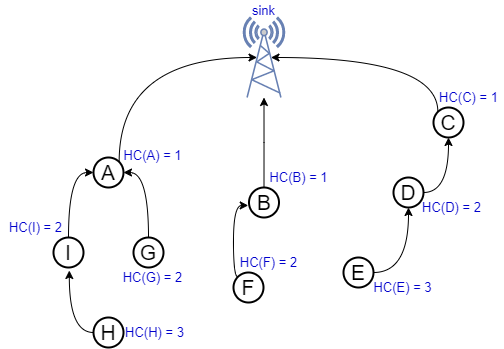
\includegraphics[width=1.1\linewidth]{Contents/Images/graphs/interestDissemination/hopCount.png}
  \end{subfigure}
  \caption{Stato della rete una volta finita la fase di Interes Dissemination}
  \label{fig:hopCount}
\end{figure}

Una volta terminata interamente la fase di \textit{Interest Dissemination}, lo stato della rete è quello mostrato in  \textbf{Figura \ref{fig:hopCount}} dove ogni nodo è a conoscenza della distanza tra se stesso e il sink. 

\section{Il protocollo GreenWUP}
GreenWUP, presentato in \cite{greenWup}, è un protocollo \textit{cross-layer} (Routing + MAC) usato nelle \textit{Green Wireless Sensor Network} che fa uso di tecnologie come \textit{energy-harvesting}, \textit{wake-up radio} e \textit{semantic-addressing} al fine di migliorare il consumo energetico della rete e in generale le sue prestazioni.  \\

GreenWUP è un protocollo \textit{converge-casting} basato sugli \textit{hop-count}. Infatti, è molto importante che ogni nodo della rete sia a conoscenza della propria distanza dal sink in termini di hop.\\
Questo valore, nel caso di GreenWUP, è calcolato automaticamente, infatti, conoscendo il raggio di azione delle 2 antenne (principale e di wake-up) e conoscendo la posizione esatta dei nodi è possibile stabilire per ogni nodo la sua distanza dal sink.\\

Tuttavia per questo progetto si è deciso di calcolare questo valore mediante un prima fase iniziale chiamata \textit{Interest Dissemination} usando il protocollo \textit{FloodWUP}.\\

Altra caratteristica molto importante per il corretto funzionamento di GreenWUP è che ogni nodo ha associato, all'interno di una stessa rete, due indirizzi di wake-up:
\begin{enumerate}
    \item \textbf{w\textsubscript{ID}}, un indirizzo statico che identifica univocamente il nodo all'interno della rete 
    \item \textbf{w\textsubscript{LE}}, un indirizzo dinamico con semantica che identifica lo stato in cui un nodo si trova in un determinato istante
\end{enumerate}
L'indirizzo \textbf{w\textsubscript{ID}} è un semplice intero progressivo che identifica i vari nodi assegnando un ID da \textit{0} a \textit{n} se si hanno \textit{n} nodi.\\
L'indirizzo \textbf{w\textsubscript{LE}}, invece, è ricalcolato periodicamente in quanto deve rappresentare lo stato attuale del nodo. In particolare è formato da due sequenze \(w_{L}w_{E}\) dove w\textsubscript{L} è la codifica del valore di hop-count del nodo e w\textsubscript{E} è l'energia residua del nodo. Nello specifico i vari livelli di energia sono discretizzati in \textit{k} classi\footnote{Ogni classe comprende un range di valori di energia, per cui un nodo con energia residua \textit{x} appartiene alla classe \textit{k} sse \(energiaResidua(nodo)\in range(\texitf{k})\)} per cui w\textsubscript{E} è la classe energetica a cui, attualmente, il nodo appartiene.\\

\'E possibile dividere in fasi l'invio di un  pacchetto DATA, inviato ovviamente da un nodo \textit{sender}\footnote{Nodo che detiene un pacchetto DATA da inoltrare verso il \textit{sink}} verso il \textit{next-hop}\footnote{Nodo vicino al \textit{sender} che riceve il pacchetto DATA da questo}:
\begin{itemize}
    \item \textit{Relay Selection}: in questa prima fase il sender prova ad instaurare una comunicazione con i receiver\footnote{Nodi vicini del sink che potrebbero essere scelti come \texitit{next-hop} }. Infatti si utilizza l'indirizzo di wake-up \textbf{w\textsubscript{LE}}. Questa procedura si considera conclusa nel momento in cui il nodo sender ha scelto, tra i propri vicini, chi sarà il next-hop.
    \item \textit{Send DATA}: in questa fase il nodo sender sollecita, mediante l'indirizzo di wake-up \textbf{w\textsubscript{ID}}, il next-hop e procede poi con l'invio del pacchetto DATA.
    \item \textit{Send ACK}: in questa fase finale il nodo next-hop, dopo aver correttamente ricevuto il pacchetto DATA, invia un ACK al nodo sender in modo da confermare la ricezione.
\end{itemize}
Un'osservazione importante è che se il next-hop si trova a distanza 1 dal sink, la fase di \textit{Relay Selection} viene saltata. Infatti il nodo sink è sempre in ascolto per cui si procede direttamente con l'invio del pacchetto DATA e con il successivo pacchetto ACK.\\\\

\begin{figure}[h!]
  \begin{subfigure}[t]{.8\linewidth}
    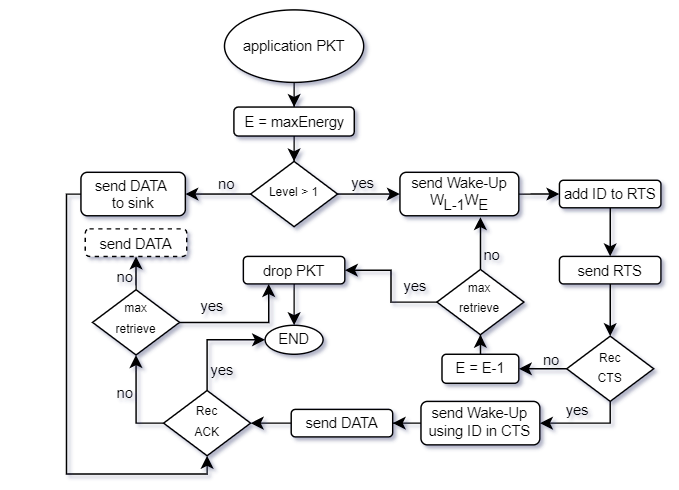
\includegraphics[width=1.15\linewidth]{Contents/Images/schemes/greenWupBase/GreenWup_base_sender.png}
  \end{subfigure}
  \caption{Logica funzionamento nodo \texitit{sender}}
  \label{fig:logicaSender}
\end{figure}

La \textbf{Figura \ref{fig:logicaSender}} sopra riportata mostra il comportamento di un nodo sender una volta che questo ha un pacchetto DATA da gestire.\\

Bisogna precisare che il nodo sink si occuperà della sola ricezione di pacchetti DATA per cui mai per nessun motivo il sink eseguirà questa procedura.\\
Come mostrato dalla \textbf{Figura \ref{fig:logicaSender}}, all'inzio la classe di energia considerata è la massima. A questo punto se il nodo è un vicino del sink, per cui \(level=1\), si salta come già detto la fase di Relay Selection e si invia direttamente il dato al sink. Altrimenti vengono sollecitati i vicini in base alla loro distanza dal sink e alla loro classe energetica. Si noti che il sender memorizza all'interno del pacchetto RTS il proprio indirizzo univoco in modo da essere ricontattato poi per ricevere il CTS.\\
Qualora non dovesse ricevere nessun pacchetto CTS, il sender riproverebbe con una classe energetica più bassa un numero massimo di volte, per poi eliminare il pacchetto e terminare la procedura.\\
Se, invece, il nodo sender dovesse ricevere il pacchetto CTS, solleciterebbe il vicino usando l'indirizzo univoco contenuto all'interno del CTS per poi mandaere il pacchetto DATA e successivamente si metterebbe in attesa dell'acknowledge. Se il nodo riceve l'ACK allora conclude la procedura, altrimenti ritenta l'invio del pacchetto per un massimo numero di volte per poi eliminarlo e terminare la procedura.\\\\

\begin{figure}[h!]
  \begin{subfigure}[t]{.8\linewidth}
    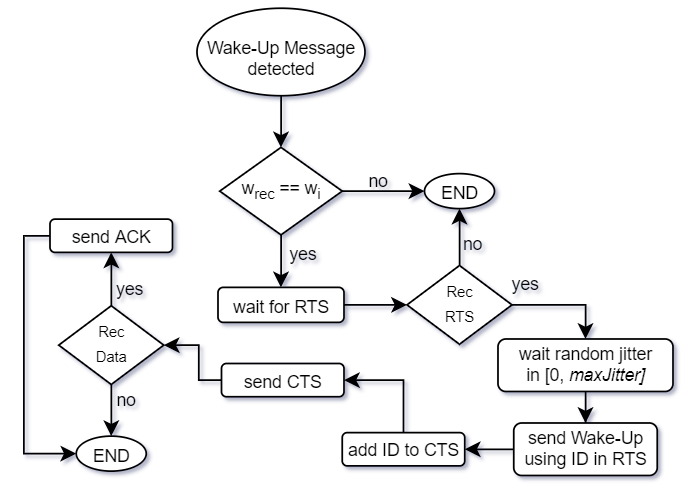
\includegraphics[width=1.1\linewidth]{Contents/Images/schemes/greenWupBase/GreenWup_base_receiver.png}
  \end{subfigure}
  \caption{Logica funzionamento nodo \texitit{receiver}}
  \label{fig:logicaReceiver}
\end{figure}

La \textbf{Figura \ref{fig:logicaReceiver}} sopra riportata mostra il comportamento di un nodo receiver una volta che questo viene sollecitato da un vicino tramite un messaggio di wake-up.\\
La prima cosa che fa un nodo receiver è controllare che la sequenza di wake-up con cui è stato sollecitato corrisponda a \(w_{i}\) dove \(w_{i} \in (w_{ID}, w_{LE})\). Se così non dovesse essere allora ignora il pacchetto e la procedura finisce, altrimenti si mette in attesa di un pacchetto RTS da parte del sender. Una volta ricevuto si aspetta un tempo calcolato randomicamente per poi sollecitare il nodo sender usando le informazioni contenute nel pacchetto RTS. Una volta sollecitato il nodo sender, il receiver procede con la creazione del pacchetto CTS con le proprie informazioni e, una volta creato, lo invia al sender.\\
A questo punto il receiver non può far altro che mettersi in attesa del pacchetto DATA. Ovviamente solo il receiver scelto come \textit{next-hop} riceverà il pacchetto DATA, per poi proseguire con l'invio dell'acknowledge. Per tutti gli altri scatterà un \textit{timeout} che terminerà la procedura.

\newpage

\section{Problematiche GreenWUP}
In questo paragrafo descriverò problematiche derivanti da mie osservazioni o da determinati risultati ottenuti durante il testing della versione base del protocollo.\\

Una prima osservazione ricade sulla fase di Relay-Selection e quindi sullo scambio dei pacchetti RTS/CTS con i wake-up message e tempi che ne derivano. GreenWUP, infatti, prevede che ad ogni nuovo pacchetto data, il nodo sender debba scegliere tra i propri vicini il next-hop che si occuperà di inoltrare il pacchetto verso il sink. Ovviamente questa è la procedura che più richiede tempo e spreco di energia per cui ripeterla sempre potrebbe essere inefficace soprattutto in scenari con traffico denso. Potrebbe, quindi, avere senso tenere traccia in qualche modo delle varie scelte che i nodi sender fanno durante l'intera simulazione in modo da ridurre il numero di ripetizioni di questa procedura.\\

Una seconda osservazione, strettamente collegata alla prima, ricade sul fatto che dall'altra parte i nodi receiver, una volta ricevuta una stringa di wake-up, non hanno nessuna logica decisionale riguardo l'attivarsi o meno in ascolto, infatti, da protocollo attivano la main radio in RX.\\
Ovviamente ciò comporta che in fase di Relay-Selection, ad esempio, tutti i receiver partecipano alla fase e, dato che solo uno poi sarà scelto come next-hop, tutti gli altri nodi non faranno altro che sprecare energia inutilmente. Se invece potessero decidere di non partecipare alla fase, evitando quindi di settare la radio principale a RX, potrebbero risparmiare energia. Ovviamente questo è un aspetto abbastanza complesso su cui bisogna prestare attenzione nello scegliere le condizioni con il quale un nodo decide o meno di attivarsi in RX o meno, in quanto potrebbe capitare che nessun nodo decida di partecipare alla fase di Relay-Selection rischiando non solo ripetizioni della fase, ma anche la perdita del pacchetto se dovesse essere raggiunto il limite di tentativi.\\

Infine, studiando l'implementazione della versione base del protocollo si può notare come ogni nodo receiver aspetti un Jitter puramente randomico prima di inviare il pacchetto CTS al sender. Potrebbe risultare utile sfruttare al meglio questo valore calcolandolo non randomicamente ma in funzione dell'energia residua, come succede in \textbf{GreenRoutes}\cite{greenRoutes}. In questo modo il nodo sender riceverebbe il pacchetto CTS dal nodo con più energia e, dato che viene scelto il primo CTS ricevuto, si eviterebbe di scegliere come next-hop un nodo al limite della classe energetica corrente.

\chapter{Modifiche e Varianti}
In questo capitolo saranno descritte delle idee riguardo miglioramenti che sono stati introdotti alla logica di GreenWUP. Nello stesso capitolo viene trattata anche l'implementazione di queste varianti.

\section{Auto-WakeUp}
Questa particolare variante va a modificare la "\textit{logica}" del protocollo relativa al nodo \textit{sender} (ovvero il nodo che detiene un pacchetto DATA da esso generato o ricevuto precedentemente, che ora deve inoltrare verso il \textit{sink}). \\
In particolare il nodo \textit{sender} è in grado di ricevere i vari CTS dai suoi vicini "svegliandosi da solo" poco prima della ricezione del primo pacchetto e di conseguenza non è più richiesto che i vari \textit{receiver} inviino prima un messaggio di wake up. \\

Questa nuova procedura ha inizio subito dopo l'invio del pacchetto RTS da parte del sender. Infatti, dopo aver eseguito le classiche istruzioni previste dall'algoritmo base (tra cui il SET\_STATE a SLEEP della main radio ovviamente) si avvia un timer chiamato \textit{TURN\_ON\_MAIN\_RADIO} (\textbf{riga 5, Codice \ref{code:afterRTS}}).

\begin{listing}[h]
    \caption{Avvio timer per svegliarsi da solo}
    \label{code:afterRTS}
    \begin{minted}[mathescape, linenos, numbersep=10pt, gobble=0, fontsize=\small, frame=lines, framesep=2mm]{cpp}

case PKT_GREEN_WUP_RTS: {
  .
  .  altre operazioni 
  .
  setTimer(TURN_ON_MAIN_RADIO, setRxAfterWaken);
  break;
}

    \end{minted}
\end{listing} \\

Questo timer scatta dopo \textit{"setRxAfterWaken"} ms per cui è molto importante che questo tempo, in cui il nodo è in SLEEP, non sia nè troppo lungo (si perderebbero uno o più pacchetti CTS) nè troppo corto (il nodo starebbe per troppo tempo in RX sprecando energia inutilmente). \\
In questa implementazione, il tempo che il nodo \textit{sender} aspetta prima di attivare la main radio, deve tener conto del tempo richiesto dal nodo per attivarsi in RX e del tempo richiesto da un potenziale \textit{relay} per attivarsi in TX, aspettare un tempo randomico chiamato \textit{jitter} (che varia da un minimo di 0 a un max definito come \textit{ctsMaxJitter}) e mandare il pacchetto CTS (formula finale in \textbf{Codice \ref{code:setRxAfterWaken}}).

\begin{listing}[h]
    \caption{Tempo che permette la ricezione del primo pacchetto CTS}
    \label{code:setRxAfterWaken}
    \begin{minted}[mathescape, linenos, numbersep=10pt, gobble=0, fontsize=\small, frame=lines, framesep=2mm]{cpp}

setRxAfterWaken = 
  + radioModule->transition[SLEEP][RX].delay
  + radioModule->transition[SLEEP][TX].delay
  + TIME_TO_SEND_CTS;

    \end{minted}
\end{listing} \\

Una volta scattato questo timer, si imposta la main radio in RX e subito dopo si pianifica, tramite il timer \textit{"TIMER\_RX\_AFTER\_WUR"} (\textbf{riga 4, Codice \ref{code:turnOff}}), lo spegnimento della main radio.

\begin{listing}[h]
    \caption{Timer che sveglia automaticamente il nodo}
    \label{code:turnOff}
    \begin{minted}[mathescape, linenos, numbersep=10pt, gobble=0, fontsize=\small, frame=lines, framesep=2mm]{cpp}

case TURN_ON_MAIN_RADIO: {
  if( !isSink ){
    toRadioLayer(createRadioCommand(SET_STATE, RX));
    setTimer(TIMER_RX_AFTER_WUR, ctsMaxJitter);
    collectOutput("MAC", "Waked-up");
  }
  break;
}

    \end{minted}
\end{listing} \\

Questo timer scatta dopo \textit{"ctsMaxJitter"} in quanto dal momento dell'invio del pacchetto RTS, prima di attivare la main radio, il nodo \textit{sender} aspetta un tempo che considera i tempi necessari per l'invio del CTS con il minimo jitter possibile (0) per cui una volta passato questo tempo deve restare in RX mode per un tempo che permetta la ricezione di un pacchetto il quale jitter è stato massimo (ctsMaxJitter). \\

Ovviamente nel momento in cui il nodo \textit{sender} riceve un CTS, questo elimina il timer \textit{"TIMER\_RX\_AFTER\_WUR"} e provvede a spegnere immediatamente l'antenna principale ignorando così tutti gli altri CTS e risparmiando di conseguenza energia. 

\section{Relay-Caching}
Con questa variante si agisce ancora una volta principalmente sui nodi \textit{sender}.\\
Infatti, i vari nodi della rete hanno la possibilità di memorizzare l'ultimo vicino scelto come next-hop in precedenza e sceglierlo nuovamente per inoltrare un eventuale nuovo dato evitando, di fatto, il classico scambio di pacchetti RTS/CTS che invece avviene per ogni pacchetto data nella versione base del protocollo.\\

L'idea nasce dopo un'attenta analisi di molte simulazioni (eseguite su diversi scenari) del protocollo GreenWUP base. In particolare, dai risultati di queste simulazioni, si nota che difficilmente un nodo \textit{x} invia un primo pacchetto data a un nodo \textit{y} e successivamente invia un altro pacchetto data a un nodo \textit{z}. Infatti quello che succede nella larghissima maggioranza dei casi analizzati è che i nodi tendono a scegliere tra i vicini sempre gli stessi next-hop.\\
Ovviamente non è sempre così, infatti, potrebbe capitare che il vicino appena scelto non può essere riscelto perché non è più disponibile o perché è impegnato nella gestione di un altro pacchetto.\\

Tuttavia, l'uso per un periodo di tempo dello stesso next hop, è quanto solitamente accade e questo è motivato dagli stessi criteri di scelta del next hop relay basati su una metrica (l'hop count) che varia molto lentamente e su metriche prestazionali dinamiche, quali la classe di energia residua, che comunque richiedono un certo tempo prima che si creino delle significative modifiche. Ha quindi senso esplorare la possibilità di ridurre i processi di selezione del next hop relay, utilizzando il caching della selezione, magari perdendo in ottimalità in sporadiche scelte di relay.\\
\\
Per l'implementazione di questa nuova funzionalità sono state definite delle nuove variabili:
\begin{listing}[h]
    \caption{Dichiarazione nuove variabili necessarie a Relay-Caching}
    \label{code:setNewVar}
    \begin{minted}[mathescape, linenos, numbersep=10pt, gobble=0, fontsize=\small, frame=lines, framesep=2mm]{cpp}

int txTimes_Cached;
int txBeforeChangingRelayCached;
string relayCachedWurAddress;
int relayCachedAddress;

    \end{minted}
\end{listing}\\
Queste nuove variabili sopra definite rappresentano rispettivamente :
\begin{enumerate}
    \item Il numero di volte in cui c'è stata una trasmissione verso il nodo cached 
    \item Il numero massimo di trasmissioni consentite verso il nodo cached
    \item L'indirizzo univoco di wake-up del nodo cached
    \item L'ID in rete del nodo cached
\end{enumerate}
\\
Si è scelto di fissare un numero massimo di invii mediante l'utilizzo del nodo cached (\textit{txBeforeChangingRelayCached}) in quanto utilizzando molte volte i vicini che i vari sender hanno in cache, questi rischiano di terminare l'energia a disposizione prima rispetto agli altri nodi. Imponendo un numero massimo di utilizzi, ovviamente si va a regolare un minimo l'utilizzo del caching affinché non si proceda sempre verso lo stesso percorso e cercando di ottenere un consumo energetico più omogeneo possibile tra i vari nodi della rete. In particolare si permette la trasmissione verso il nodo cached per un massimo di 3 volte \footnote{Valore ottimizzato dopo svariate simulazioni con diverse quantità}.\\

La variabile \textit{txBeforeChangingRelayCached}, inoltre, non comprende solo gli invii di pacchetti data usando il nodo cached, ma comprende in generale tutte le trasmissioni verso il nodo cached.\\
Potrebbe infatti succedere che un nodo cached non sia raggiungibile (per motivi legati all'energia residua o altri). In questo caso, ovviamente, il nodo sender ritenta l'invio un numero \textit{x} di volte.\\
Accumulando in una stessa variabile (\textit{txTimes\_Cached}) sia gli invii riusciti che le eventuali ritrasmissioni si riesce a "scoraggiare" l'invio verso quel vicino.\\

Ovviamente quando \textit{txTimes\_Cached} supera in valore \textit{txBeforeChangingRelayCached} si procede esattamente come il protocollo base prevede, ovvero, con lo scambio di RTS e CTS.\\

La nuova procedura ha inizio poco prima dell'invio del primo messaggio di wake-up in broadcast prima dell'RTS da parte del sender.

\begin{listing}[h]
    \caption{Scelta tra invio mediante relay o invio classico}
    \label{code:checkForRelay}
    \begin{minted}[mathescape, linenos, numbersep=10pt, gobble=0, fontsize=\small, frame=lines, framesep=2mm]{cpp}

if( relayCachedAddress != -1 && 
  txTimes_Cached < txBeforeChangingRelayCached){
	
  txTimes_Cached++;
  relayAddress = relayCachedAddress;	
  setState(MAC_STATE_SENDING_DATA);

  sendWurAddress( relayCachedWurAddress);
} else {
  txTimes_Cached = 0;
		
  # scambio RTS/CTS come da versione base #
}

    \end{minted}
\end{listing} \\

Con la nuova funzionalità, prima di inviare il messaggio di wake-up in broadcast e procedere con lo scambio di RTS/CTS, il nodo controlla che non sia presente un nodo in cache (\textbf{riga 1, Codice \ref{code:checkForRelay}}) e che non siano state superate le trasmissioni massime verso questo (\textbf{riga 2, Codice \ref{code:checkForRelay}}).\\
\\
Se così fosse, incrementa il numero di trasmissioni effettuate e procede con l'inivio del messaggio di wake-up usando l'indirizzo di wake-up univoco del nodo cached.\\

Ovviamente, durante l'invio del primo pacchetto data gestito da un determinato nodo \textit{x}, non sarà presente nessun nodo in cache per cui si procede con lo scambio classico dei pacchetti RTS/CTS.\\
Alla ricezione del primo pacchetto CTS (e quindi quando normalmente un sender sceglie il next-hop), il nodo provvede a memorizzare informazioni quali indirizzo di wake-up univoco e ID in rete del nodo che ha inviato il CTS.

\begin{listing}[h]
    \caption{Memorizzazione di un nuovo relay node}
    \label{code:cachingNode}
    \begin{minted}[mathescape, linenos, numbersep=10pt, gobble=0, fontsize=\small, frame=lines, framesep=2mm]{cpp}

relayCachedWurAddress = genericPkt->getWurAddress();
relayCachedAddress = genericPkt->getSource();

    \end{minted}
\end{listing} \\

Dall'altra parte, invece, i vicini del nodo sender devono essere in grado di capire quando sono svegliati dalla procedura di scambio RTS/CTS oppure sono stati svegliati in qualità di nodi cached.\\
Per capire se un nodo è stato cached, ogni volta che questo riceve un messaggio di wake-up controlla che l'indirizzo di wake-up corrisponda al suo indirizzo di wake-up univoco e inoltre deve trovarsi nello stato: \textit{MAC\_STATE\_IDLE}. \\
Se tutte le condizioni sono rispettate, il nodo imposta il proprio stato in \textit{MAC\_STA-} \textit{TE\_WAIT\_FOR\_DATA}.

\begin{listing}[h]
    \caption{Procedura con cui un nodo capisce di essere cached}
    \label{code:detectWUM}
    \begin{minted}[mathescape, linenos, numbersep=10pt, gobble=0, fontsize=\small, frame=lines, framesep=2mm]{cpp}

if( strcmp(myUniqueWurAddress.c_str(), name) == 0 &&
    state == MAC_STATE_IDLE ){
    
  setState(MAC_STATE_WAIT_FOR_DATA);
}

    \end{minted}
\end{listing} \\

Quest'ultima condizione è necessaria in quanto potrebbero esserci dei problemi quando un nodo sender avvia la procedura di scambio RTS/CTS e riceve il messaggio di wake-up che preannuncia un CTS. Se non ci fosse questa condizione, il nodo sender setterebbe il proprio stato in \textit{MAC\_STATE\_WAIT\_FOR\_DATA}, ignorando il pacchetto CTS ricevuto. \\

Altro problema che potrebbe avere un nodo cached è che non avendo ricevuto prima del pacchetto data il classico RTS, non sa effettivamente da chi sta per ricevere quest'ultimo pacchetto, per cui non sarebbe in grado di inviare poi l'acknowledgement al nodo sender.\\
Per fare ciò, un nodo che riceve un pacchetto data effettua un controllo molto semplice sulle variabili che dovrebbero contenere le informazioni relative al nodo sender e nel caso le imposta prendendole dal pacchetto data appena ricevuto.

\begin{listing}[h]
    \caption{Procedura con cui un nodo cached riconosce il nodo sender}
    \label{code:setForACK}
    \begin{minted}[mathescape, linenos, numbersep=10pt, gobble=0, fontsize=\small, frame=lines, framesep=2mm]{cpp}

if( genericPkt->getSource() != senderAddress && 
    !isSink && 
    senderAddress == -1 ){

  senderWurAddress = genericPkt->getWurAddress();
  senderAddress = genericPkt->getSource();
}

    \end{minted}
\end{listing} \\

\'E molto importante che la variabile \textit{senderAddress} sia uguale a -1 in quanto questo evita di prendere in considerazione pacchetti data che in realtà non sono destinati a quel nodo. Infatti nel caso della procedura di invio con il nodo cached, questo sarà in \textit{WAIT\_FOR\_DATA} e non avrà le informazioni relative al sender; nel caso invece della classica procedura, quando un nodo relay sta in \textit{WAIT\_FOR\_DATA} conosce già chi sta per mandare il pacchetto data (avendo ricevuto il pacchetto RTS).

\section{All-in-One}
Alla luce di quanto presentato fino ad ora, si presenta una terza versione in cui le due modifiche sopra presentate coesistono. \\
Semplicemente la logica di funzionamento di questa nuova proposta consiste nell'unione delle due sopra descritte.\\
\'E possibile vedere i risultati in \textbf{Figura \ref{fig:final}}.\\

\section{All-in-One 2.0}
Con questa nuova variante si propone una versione aggiornata di \textbf{\textit{All-in-One}}.\\
\\
In particolare si è deciso di agire sugli aspetti più deboli di \textit{All-in-One} e in generale del protocollo base GreenWUP.\\
Infatti con queste nuove modifiche è cambiato sia la semantica del tempo \textit{Jitter} di ogni \textit{receiver} sia la logica con cui viene impostato il numero di trasmissioni verso un nodo cached.

\subsection{Semantica del tempo Jitter}
Come succedeva per tutte le varianti proposte finora, compresa la versione base del protocollo, il tempo Jitter che ogni receiver aspetta prima di inviare il pacchetto CTS è calcolato in modo puramente aleatorio. Come già discusso questa soluzione non è delle migliori per cui si è deciso di attribuirgli una semantica più interessante.\\
In particolare ogni receiver calcola un tempo jitter considerando la quantità di energia utilizzabile. In questo modo il nodo sender riceverà molto probabilmente il primo pacchetto CTS non da un nodo qualunque ma dal nodo con più energia disponibile.\\
La nuova formula che definisce il tempo Jitter è quindi la seguente:
\[Jitter = \delta_{d} * (1-\delta_e) + \delta_r\]
con \(\delta_{d}\) che rappresenta il massimo delay consentito, \(\delta_{e}\) rappresenta la percentuale di energia attualmente disponibile normalizzata in \([0-1]\) e \(\delta_{r}\) che rappresenta, invece, un valore randomico.\\

\'E facile notare che adesso il valore finale di \textit{Jitter} dipende fortemente dal valore energetico che un nodo ha in un determinato istante. In particolare, minore è la percentuale di energia maggiore sarà il Jitter. La presenza di \(\delta_{r}\) è richiesta in quanto consente di evitare le collisioni nel momento in cui ci siano più nodi receiver con la stessa percentuale di energia.

\subsection{Decisione del numero di trasmissioni verso il nodo cached}
\'E stata inoltre modificata anche la logica con cui viene valorizzata la variabile \textit{txBeforeChangingRelayCached}.\\
Inizialmente, infatti, questa variabile, che regola in numero di trasmissioni verso il nodo cached (\textbf{riga 2, Codice \ref{code:checkForRelay}}), era stata impostata staticamente\footnote{Valore scelto ovviamente dopo una serie di tentativi, osservando i risultati ottenuti con vari valori.} a 3.\\
Grazie alle modifiche apportate ogni nodo è in grado di decidere ogni volta il numero di trasmissioni verso un determinato nodo cached basandosi su parametri che forniscono una valutazione del nodo cached. In questo modo è stato possibile aumentare il numero di utilizzi per quei nodi in grado di supportare l'incarico, mentre per altri nodi si è scelto un valore più basso in modo da evitare che questi esaurissero la propria energia.\\ 

Per fare ciò è stata necessaria la modifica al Jitter sopra descritta. Infatti, un nodo sender decide di impostare questo valore basandosi sul tempo che i vari receiver impiegano ad inviare il pacchetto CTS e, dato che questo dipende dalla loro energia residua, si può affermare che maggiore sarà l'energia del nodo receiver (di conseguenza minore sarà il Jitter calcolato) maggiore sarà anche il numero di trasmissioni che il nodo sender decide di fare verso il nodo cached in questione.\\

Nonostante il numero di trasmissioni sia variabile tra i vari nodi sender si è scelto comunque di fissare un tetto massimo, e ovviamente minimo, affinché non si concentri il traffico sempre verso gli stessi nodi.\\ Questo fenomeno potrebbe infatti risultare dannoso in scenari in cui c'è poco traffico e quindi si utilizzerebbero per tutto il lifetime della rete gli stessi next-hop.\\
In particolare il numero di ritrasmissioni che il sender sceglierà per un determinato nodo cache apparterrà all'intervallo \([1, 6]\).\\
Per la realizzazione di questa modifica sono, inoltre, state usate 3 nuovi variabili:

\begin{listing}[h]
    \caption{Nuove variabili usate per le modifiche}
    \label{code:variables_final2.0}
    \begin{minted}[mathescape, linenos, numbersep=10pt, gobble=0, fontsize=\small, frame=lines, framesep=2mm]{cpp}

double maxTxCache;
double minTxCache;
double factorTxCache = (minTxCache - maxTxCache) / 5;

    \end{minted}
\end{listing}\\

In particolare queste variabili aiutano a definire un mapping tra i tempi di attesa dei pacchetti CTS e l'intervallo \([1, 6]\) sopra citato:
\begin{itemize}
    \item \textit{maxTxCache} è un valore definito inizialmente da ogni nodo, calcolato usando la formula del Jitter ma considerando la massima energia. Questo valore corrisponde al migliore dei casi, ovvero, l'estremo superiore dell'intervallo, 6;
    \item \textit{minTxCache} è anch'esso calcolato inizialmente da tutti i nodi usando la formula del Jitter ma questa volta si considera solo il 50\% dell'energia disponibile. Questo corrisponde al caso "peggiore", infatti è associato all'estremo inferiore dell'intervallo, 1;
    \item \textit{factorTxCache} è invece un valore che permette di dividere l'intervallo\\ \([maxTxCache, minTxCache]\) nelle stesse parti dell'intervallo \([1, 6]\) in modo da avere un mapping corretto per ogni valore.
\end{itemize}

A questo punto, quando un nodo cached, durante la fase di Relay-Selection, riceve il pacchetto CTS da un vicino, dopo averlo memorizzato in cache, calcola anche il numero di trasmissioni da affidare a quest'ultimo usando la seguente funzione:

\begin{listing}[h]
    \caption{Funzione che restituisce il corretto numero di ritrasmissioni per un nodo cached}
    \label{code:getTxTimes_final2.0}
    \begin{minted}[mathescape, linenos, numbersep=10pt, gobble=0, fontsize=\small, frame=lines, framesep=2mm]{cpp}

int GreenWup::getTxTimes(double x) {
  if( x <= maxTxCache ) return 6;
  if( x >= minTxCache) return 1;

  int n = 7;
  double temp = maxTxCache;
  
  while(x > temp){
    temp += factorTxCache;
    n--;
  }
  return n;
}

    \end{minted}
\end{listing}\\

La funzione illustrata nel \textbf{Codice \ref{code:getTxTimes_final2.0}} prende in input un valore \textit{x} definito come il tempo trascorso tra l'invio del pacchetto RTS e la ricezione del pacchetto CTS\footnote{ovviamente eliminando tempi noti come quello necessario all'invio del CTS} e restituisce un intero \textit{n} appartenente all'intervallo \([1, 6]\), a seconda, ovviamente, della posizione di \textit{x} nell'intervallo \([maxTxCache, minTxCache]\).\\
\\

\newpage

Per completezza la \textbf{Figura \ref{fig:getTxTimes_final2.0}} mostra graficamente in che modo la funzione appena presentata restituisce un valore \textit{n} dato un valore in input \textit{x}.

\begin{figure}[h!]
  \begin{subfigure}[t]{0.9\linewidth}
    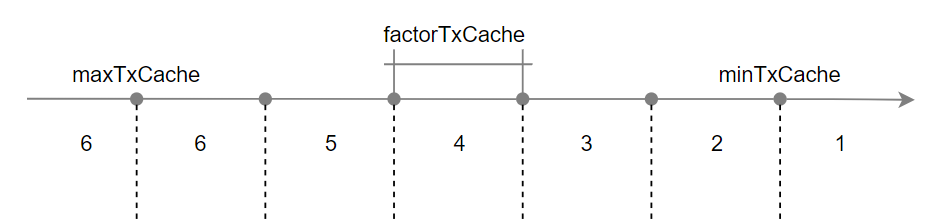
\includegraphics[width=1.1\linewidth]{Contents/Images/schemes/final2.0/getTxTrasmiss.PNG}
    \caption{TX Time for the WUR}
  \end{subfigure}
  \caption{Grafico dei valori di ritorno della funzione getTxTimes}
  \label{fig:getTxTimes_final2.0}
\end{figure}

\chapter{Valutazione Prestazionale}
In questo capitolo sarà descritto il simulatore utilizzato per il confronto tra la versione base del protocollo e le varie varianti sopra descritte. Sarà anche fornita una descrizione dei vari scenari usati per le simulazioni. Saranno infine presentati i risultati della valutazione prestazionale effettuata.

\section{Il Simulatore: GreenCastalia}
Le varie simulazioni sono state eseguite utilizzando il simulatore GreenCastalia, descritto in \cite{gCastalia}. \\
GreenCastalia è un'estensione open-source per il più popolare simulatore Castalia \cite{castalia} che consente di gestire scenari in cui i vari nodi che compongono la rete sono integrati con dispositivi di raccolta di energia (\textit{energy harvesting capabilities}).\\
In particolare è stata usata un'estensione di GreenCastalia che supporta la tecnologia delle wake-up radios.

\section{Scenario e Configurazione Simulatore}
Lo scenario di simulazione prevede un'area utile ai nodi di 100x100 metri su cui 139 dei 140 nodi totali sono distribuiti in modo randomico uniforme. \\
Il sink node (per convenzione il nodo 0) è l'unico nodo della rete con posizione fissa, in particolare è posizionato al centro dell'area (x=50, y=50). \\
Ovviamente il 100\% dei nodi è in grado di generare pacchetti DATA, fatta eccezione per il sink che si limita a riceverli.\\

Il data rate del canale, per la radio principale,  è impostato a 250 Kbps. \\
Il modello energetico considerato è quello del nodo sensoriale \textit{MagoNode}++\cite{magonode++}, ideato da SensesLab e basato sulla precedente versione \textit{MagoNode}\cite{magonode}, una piattaforma ideata per WSN che fornisce supporto a tecnologie di wake-up radio e di energy harvesting.\\

Ogni nodo della rete ha 3 diverse modalità per l'antenna principale (e ognuna ovviamente prevede un consumo più o meno alto). In particolare vi è la modalità di invio (\textit{TX}), la modalità di ricezione (\textit{RX}) e la modalità in cui l'antenna consuma molto meno energia (\textit{SLEEP}). \\

Per tutte le simulazioni effettuate, l'antenna principale è in grado di coprire un'area di raggio 60m, mentre per l'antenna di wake-up l'area coperta ha raggio 25m.
Per quanto riguarda l'energy harvesting, vengono utilizzate delle celle solari che permettono appunto di accumulare energia. \'E possibile predire la quantità di energia accumulata da ogni nodo grazie a un sistema di energy prediction che, dopo un periodo di \textit{"training"} è in grado di fornire una stima affidabile dell'energia che sarà accumulata nel breve futuro.\\

\begin{table}[h]
    \setlength\doublerulesep{1mm} 
    \begin{tabular}{ |p{8cm}|p{4cm}|  }
        \hline
        \multicolumn{2}{|c|}{\textbf{Parametri di simulazione}}\\
        \hline \hline
        \textbf{Parametro}  & \textbf{Valore}\\
        \hline
        Tempo di simulazione                            & 72h \\
        Durata allenamento degli energy predictor       & 71h \\
        Tempo utile allo scambio di pacchetti           & 1h \\
        Nodi della rete                                 & 140 \\
        Nodi che possono generare pacchetti Data        & 139 \\
        Dimensione area di simulazione                  & 100 x 100 \textit{ mt\textsuperscript{2}}\\
        Distribuzione dei nodi (1-139)                  & randomica uniforme \\
        Posizione Sink (0)                              & coord(50, 50) \\
        Jitter massimo previsto                         & 100ms \\
        Piattaforma hardware                            & MagoNode++ \\
        Raggio di azione radio principale               & 60mt \\
        Raggio di azione radio wake-up                  & 25mt \\
        Frequenza radio principale                      & 2.4GHz \\
        Frequenza radio wake-up                         & 868MHz \\
        Frequenza aggiornamento wake-up addresses       & 300s \\
        Sorgente energetica esterna                     & Energia solare \\
        Capacità massima delle batterie                 & 245000mA \\
        \hline
    \end{tabular}
    \centering
    \vspace*{5mm}
    \caption{Tabella di configurazione delle simulazioni.}
    \label{configs}
\end{table}

\section{Metriche prestazionali}
Durante l'intero progetto, le varie proposte, così come la versione base del protocollo GreenWUP, sono state valutate osservando l'andamento delle seguenti metriche:

\vspace{0.3em}

\begin{itemize}
    \itemsep0em
    \item \emph{Tx Times}, definito come il tempo che ogni nodo, in media, passa con l'antenna di wake-up in modalità TX durante l'intera simulazione;
    \item \emph{Energy Consuption}, definita come l'energia totale spesa da ciascun nodo della rete per l'invio e la ricezione dei vari pacchetti DATA e di controllo, con la sola eccezione del sink node;
    \item \emph{End-to-End Latency}, definita come il tempo che un pacchetto impiega dal momento in cui è stato generato fino al raggiungimento del sink node;
    \item \emph{Packet Delivery Ratio}, definita come la percentuale di pacchetti DATA ricevuti correttamente dal sink node sul totale dei pacchetti DATA generati dai vari nodi della rete;
\end{itemize}

\\\\

Ovviamente l'obbiettivo è quello di migliorare il più possibile questi valori e in particolare:
\begin{itemize}
    \item Minimizzare il tempo speso con la wake-up radio in modalità TX;
    \item Minimizzare l'energia totale spesa dalla rete;
    \item Minimizzare il tempo impiegato da un pacchetto per raggiungere il sink node;
    \item Massimizzare la percentuale di pacchetti DATA ricevuti correttamente dal sink node.
\end{itemize}
\newpage
\section{Valutazione sperimentale delle varianti proposte}
Per tutte le simulazioni è stata usata la configurazione nella \textbf{Tabella \ref{configs}} facendo variare ogni volta il parametro \textit{iaTime} con cui si regola il traffico in rete, infatti, i nodi generano un pacchetto DATA ogni \textit{iaTime} secondi.\\
I risultati presentati sono mediati su un numero di run sufficiente a fornire un intervallo di confidenza del 95\% con una precisione del 5\%. \\
Per ciascuna metrica viene presentata la media  ottenuta nelle simulazioni effettuate. \\
Si precisa che sono inclusi nei risultati anche i consumi energetici dovuti alla fase di \textit{interest dissemination}.


\subsection{Auto-WakeUp}
\textit{1) TX Time}: come mostrato in \textbf{Figura \ref{fig:TXTime_1}}, il tempo medio che le varie antenne di WakeUp passano in TX diminuisce in modo significativo all'aumentare del traffico in rete. Questo risultato giustifica anche quanto è possibile vedere in \textbf{Figura \ref{fig:EnergySpent_1}} in quanto  i vari nodi che ricoprono il ruolo di \textit{receiver}, e che quindi svolgono la funzione di relay per un determinato pacchetto, non inviano più il WakeUp message prima del CTS e in questo modo si vanno a risparmiare \textit{n*m} invii nel caso in cui si hanno \textit{n} potenziali nodi relay e \textit{m} pacchetti data da inviare. In questo caso i miglioramenti sono costantemente tra il 72\% e il 73\%.
\\\\
\textit{2) Energy Consuption}: come mostrato in \textbf{Figura \ref{fig:EnergySpent_1}}, si ha un miglioramento nell'energia complessiva consumata dalla rete alla fine della simulazione. In particolare si ottiene un miglioramento maggiore all'aumentare del traffico in rete, infatti, l'energia consumata diminuisce di circa 7\% nel caso in cui si genera un data packet ogni 50 secondi (circa 65 pacchetti in totale), mentre diminuisce di circa 11\% nel caso in cui si genera un data packet ogni 2 secondi (circa 1700 pacchetti in totale).
\\\\
\textit{3) End-to-End Latency}: come mostrato in \textbf{Figura \ref{fig:Latency_1}}, la latenza è un parametro che ne risente, invece, negativamente. Questo può essere dovuto al fatto che, svegliandosi da solo, il nodo mittente non riesca sempre a ricevere il primo pacchetto CTS per cui deve aspettare il prossimo. Tuttavia, la variante proposta risulta sì più lenta, ma questo ritardo varia da un massimo di 8 millisecondi fino ad un minimo di 6 millisecondi per cui non risulta essere un ritardo particolarmente problematico.
\\\\
\textit{4) Packet Delivery Ratio}: come mostrato in \textbf{Figura \ref{fig:PDR_1}}, il PDR è anch'esso un parametro che risente in modo negativo delle modifiche apportate con autoWakeUp. Dalle simulazioni, così come dal grafico, si evince una perdita di circa lo 0.5\% in più rispetto alla versione base del protocollo nel caso iaTime è 2. Nonostante il PDR più basso, la variante proposta riesce comunque a consegnare sempre almeno il 99.3\% dei pacchetti generati (contro il 99.8\% del base GreenWUP), risultato comunque accettabile nonostante la piccola perdita di qualità.

\begin{figure}[H]
  \begin{subfigure}[t]{0.49\linewidth}
    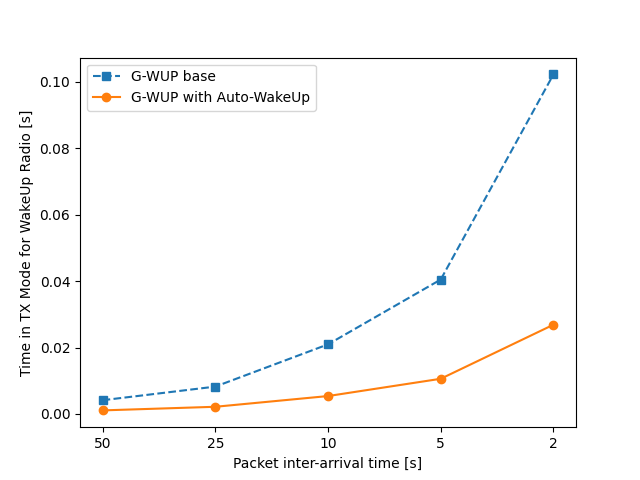
\includegraphics[width=1.1\linewidth]{Contents/Images/graphs/autoWakeUp/tx_time.png}
    \caption{TX Time for the WUR}
    \label{fig:TXTime_1}
  \end{subfigure}
  \begin{subfigure}[t]{0.49\linewidth}
    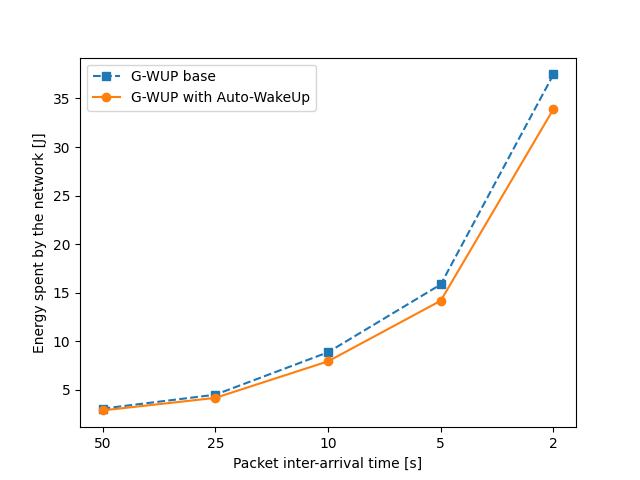
\includegraphics[width=1.1\linewidth]{Contents/Images/graphs/autoWakeUp/energySpent.png}
    \caption{Energy Consuption}
    \label{fig:EnergySpent_1}
  \end{subfigure}
  \begin{subfigure}[t]{0.49\linewidth}
    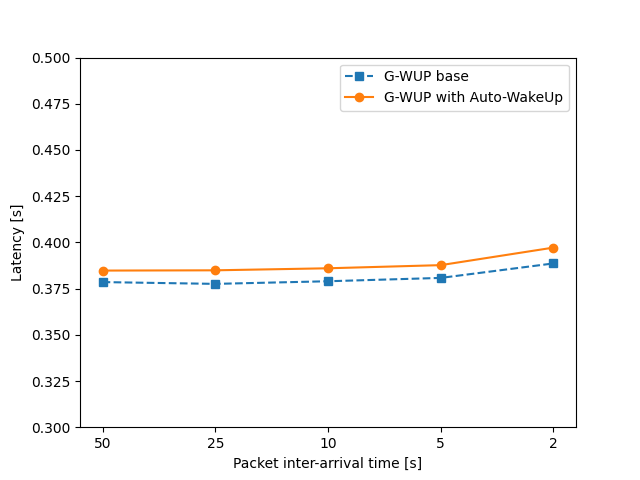
\includegraphics[width=1.1\linewidth]{Contents/Images/graphs/autoWakeUp/latency.png}
    \caption{End-to-End Latency}
    \label{fig:Latency_1}
  \end{subfigure}
  \begin{subfigure}[t]{0.49\linewidth}
    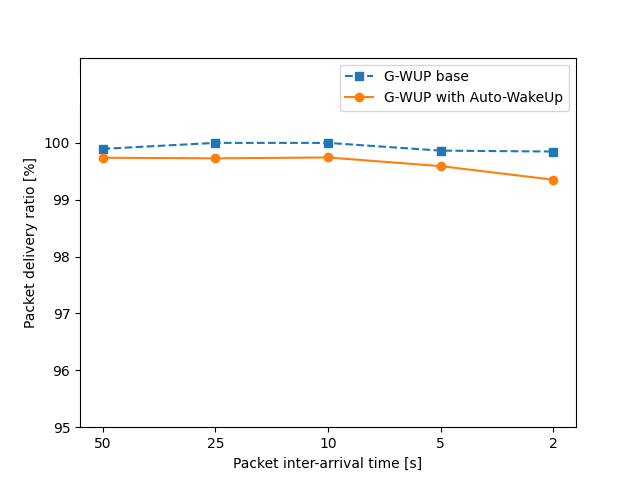
\includegraphics[width=1.1\linewidth]{Contents/Images/graphs/autoWakeUp/pdr.png}
    \caption{Packet Delivery Ratio}
    \label{fig:PDR_1}
  \end{subfigure}
  \caption{Confronto delle prestazioni tra versione base di GreenWUP (blu) e variante proposta (arancio) in termini di energia complessiva consumata, tempo in TX mode della WUR, latenza end-to-end e PDR}
  \label{fig:autoWakeUp}
\end{figure}

In sintesi, il meccanismo introdotto porta ad una ottimizzazione del tempo di trasmissione delle main radio ma non ha benefici significativi sulle
prestazioni end-to-end del sistema.
\newpage

\subsection{Relay-Caching}
Si precisa che tutti in tutti gli scenari simulati si assume che la rete sia completamente connessa per cui da un qualsiasi nodo \textit{x} è possibile raggiungere tramite uno o più nodi il nodo \textit{sink}.
\\\\
\textit{1) TX Time}: come mostrato in \textbf{Figura \ref{fig:TXTime_2}}, anche qui il tempo che in media i nodi utilizzano la wake-up Radio per trasmettere messaggi di wake-up diminuisce significativamente rispetto alla versione base di GreenWUP all'aumentare del traffico in rete. Questo è un risultato che ci si aspettava in quanto adesso i vari nodi hanno la possibilità di evitare lo scambio di pacchetti RTS/CTS con i propri vicini, che ricordiamo sono seguiti da messaggi di wake-up da e verso il nodo sender.\\
Ovviamente più pacchetti data vengono inviati e più volte si evita il classico scambio RTS/CTS, ecco perché questa variante presenta tempi in TX minori man mano che il traffico aumenta. In questo caso i miglioramenti sono tra il 50\% e il 62\%.
\\\\
\textit{2) Energy Consuption}: come mostrato in \textbf{Figura \ref{fig:EnergySpent_2}}, l'energia consumata dall'intera rete è minore rispetto l'energia consumata dalla versione base.\\
Anche in questo caso, il risultato è dovuto al fatto che ci sono molti meno scambi di RTS/CTS. In particolare questa procedura è eseguita soltanto una volta ogni quattro pacchetti data da inoltrare (dato che è possibile trasmettere verso il nodo cached per un massimo di 3 volte), inoltre, considerando che la procedura richiede l'invio di \(2 + ( 2 * n)\) pacchetti se si hanno \textit{n} possibili relay node che rispondo all' RTS del sender, è facile intuire un miglioramento nei consumi energetici di ogni nodo. I miglioramenti ottenuti sono, nel migliore dei casi (\textit{iaTime}=2), circa del 15\%. Per configurazioni con meno pacchetti si aggira invece intorno al 10-13\%.
\\\\
\textit{3) End-to-End Latency}: come mostrato in \textbf{Figura \ref{fig:Latency_2}}, non solo vi è un miglioramento rispetto la versione base di GreenWUP, ma questo fattore di miglioramento aumenta all'aumentare del traffico in rete.\\
Ovviamente questo è dovuto al fatto che in questo contesto, così come anche in altri, il concetto di \textit{caching} di informazioni dà il meglio di se in situazioni in cui il traffico è maggiore. Infatti non dovendo aspettare tempi\footnote{\'E stato citato il jitter randomico ma ovviamente ci sono anche altri tempi di attesa: ad esempio dopo l'invio di un messaggio di wake-up i nodi aspettano un tempo che permetta a chi riceve il messaggio di impostare la main radio in RX prima di mandare l'informazione.} come il jitter randomico, un nodo impiega molto meno tempo ad inoltrare un pacchetto verso un proprio vicino (se questo ovviamente è stato memorizzato in precedenza). I miglioramenti qui sono più importanti, infatti, abbiamo un miglioramento di circa il 25\% in reti molto trafficate che va a scendere fino a un minimo del 12-15\% per reti meno trafficate. 
\\\\
\textit{4) Packet Delivery Ratio}: come mostrato in \textbf{Figura \ref{fig:PDR_2}}, la percentuale di pacchetti ricevuti è paragonabile a quella della versione base, garantendo sempre la corretta ricezione di almeno il 99\% dei pacchetti.
\\\\
Ovviamente, come già detto, è molto importante per questa variante non "stressare" troppo i nodi cached in quanto se questi dovessero essere spesso non disponibili si andrebbero a fare svariate ritrasmissioni in più rispetto alla versione base, causando un degrado non sono in termini di latenza ma anche di energia consumata.\\
In questo caso, ogni nodo può trasmettere verso il nodo cached non più di 3 volte.

\begin{figure}[H]
  \begin{subfigure}[t]{0.49\linewidth}
    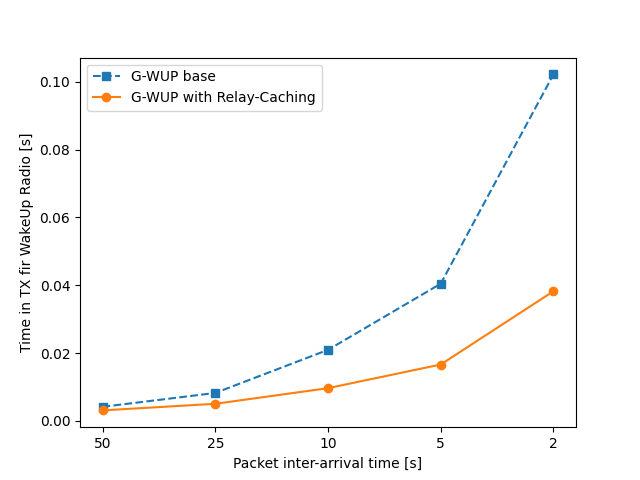
\includegraphics[width=1.1\linewidth]{Contents/Images/graphs/relayCaching/tx_time.png}
    \caption{TX Time for the WUR}
    \label{fig:TXTime_2}
  \end{subfigure}
  \begin{subfigure}[t]{0.49\linewidth}
    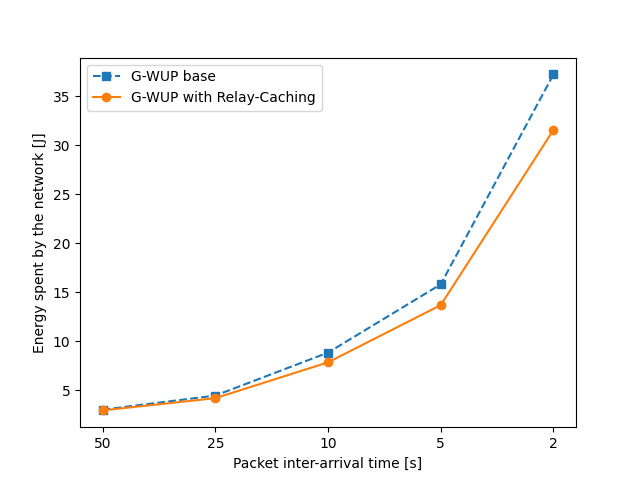
\includegraphics[width=1.1\linewidth]{Contents/Images/graphs/relayCaching/energySpent.png}
    \caption{Energy Consuption}
    \label{fig:EnergySpent_2}
  \end{subfigure}
  \begin{subfigure}[t]{0.49\linewidth}
    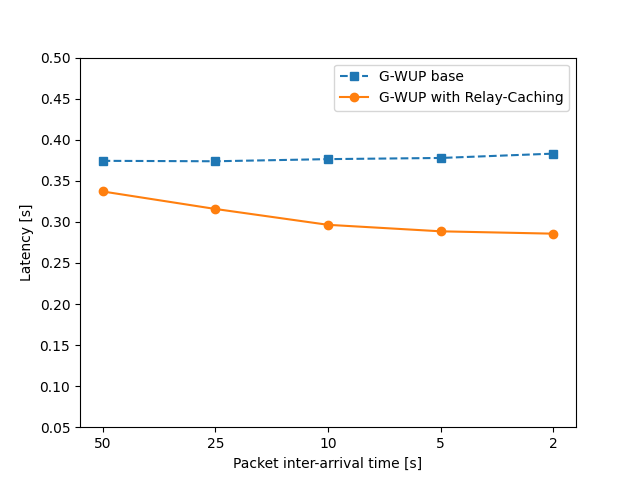
\includegraphics[width=1.1\linewidth]{Contents/Images/graphs/relayCaching/latency.png}
    \caption{End-to-End Latency}
    \label{fig:Latency_2}
  \end{subfigure}
  \begin{subfigure}[t]{0.49\linewidth}
    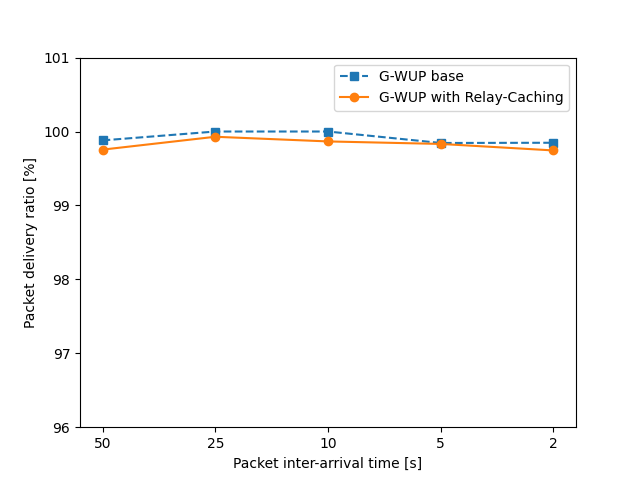
\includegraphics[width=1.1\linewidth]{Contents/Images/graphs/relayCaching/pdr.png}
    \caption{Packet Delivery Ratio}
    \label{fig:PDR_2}
  \end{subfigure}
  \caption{Confronto delle prestazioni tra versione base di GreenWUP (blu) e variante proposta (arancio)}
  \label{fig:relayCaching}
\end{figure}

In sintesi la variante che introduce il caching mostra di riuscire a ridurre significativamente il problema dell'attivazione della main radio con miglioramenti significativi in termini di energia consuma, senza degradare l'affidabilità della consegna delle informazioni. La variante riesce anche a ridurre in modo significativo le latenze, metrica importante in sistemi che, sempre piu', richiedono la rapida consegna di informazioni per supportare applicazioni "industria 4.0" o realizzare sistemi di allarme.

\subsection{All-in-One}
Si precisa che tutti in tutti gli scenari simulati si assume che la rete sia completamente connessa per cui da un qualsiasi nodo \textit{x} è possibile raggiungere tramite 1 o più nodi il nodo \textit{sink}.
\\\\
\textit{1) TX Time}: come mostrato in \textbf{Figura \ref{fig:TXTime_final}}, la versione che racchiude tutte le modifiche si comporta meglio rispetto alle altre soluzioni. Ovviamente in questo caso non solo si riduce di molto il numero di wake-up message scambiati durante la fase di relay selection, ma vengono meno tutti i wake-up message usati per sollecitare il nodo sender prima che i receiver inviino il pacchetto CTS.\\
Anche qui il coefficiente di miglioramento aumenta all'aumentare del numero di pacchetti DATA generata dai nodi della rete.\\
In particolare i miglioramenti sono del 77-80\% rispetto la versione base del protocollo GreenWUP e del 20-35\% rispetto ala variante con Auto-WakeUp.
\\\\
\textit{2) Energy Consuption}: come mostrato in \textbf{Figura \ref{fig:EnergySpent_final}}, c'è un piccolo miglioramento anche a livello di energia complessiva consumata dai nodi della rete. Ovviamente questo risultato era aspettato in quanto qui si sommano i vantaggi delle varianti di Relay-Selection e Auto-WakeUp in termini di invio di pacchetti (che siano questi di wake-up o RTS/CTS). Si ha infatti un piccolo miglioramento del 2-4\% rispetto la variante con Relay-Caching e un miglioramento totale di circa 15-18\% rispetto la versione base di GreenWUP.
\\\\
\textit{3) End-to-End Latency}: come mostrato in \textbf{Figura \ref{fig:Latency_final}}, nel caso della latenza quest'ultima variante si comporta praticamente come la versione con Relay-Caching tranne per qualche piccolo peggioramento in alcuni casi. \\
In particolare si ha un piccolo peggioramento che varia tra lo 0.5-1\% rispetto la versione con Relay-Caching mentre si ha un miglioramento del 20-26\% rispetto la versione base del protocollo GreenWUP. 
\\\\
\textit{4) Packet Delivery Ratio}: come mostrato in \textbf{Figura \ref{fig:PDR_final}}, vale quanto detto per la latenza end-to-end. Quest'ultima variante si comporta allo stesso modo della versione con Relay-Caching, presentando, di fatto, un piccolo peggioramento rispetto la versione base del protocollo GreenWUP base.\\
In particolare si ha un peggioramento dello 0.2\%, un peggioramento che non comporta grossi problemi, infatti, come tutte le altre varianti proposte, quest'ultima garantisce in media la carretta ricezione del 99.8\%.

\begin{figure}[H]
  \begin{subfigure}[t]{0.49\linewidth}
    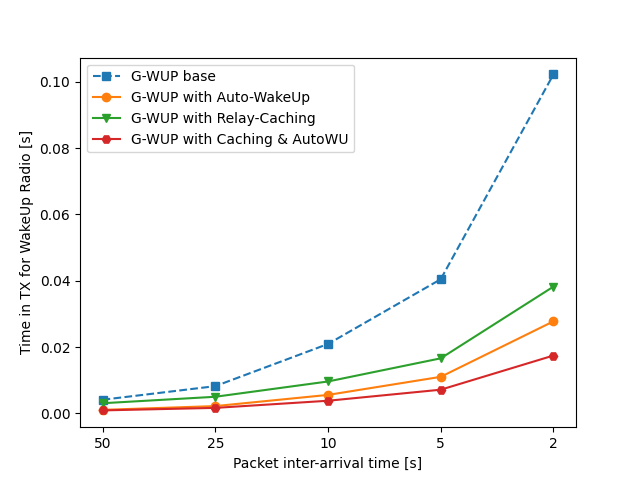
\includegraphics[width=1.1\linewidth]{Contents/Images/graphs/final/tx_time.png}
    \caption{TX Time for the WUR}
    \label{fig:TXTime_final}
  \end{subfigure}
  \begin{subfigure}[t]{0.49\linewidth}
    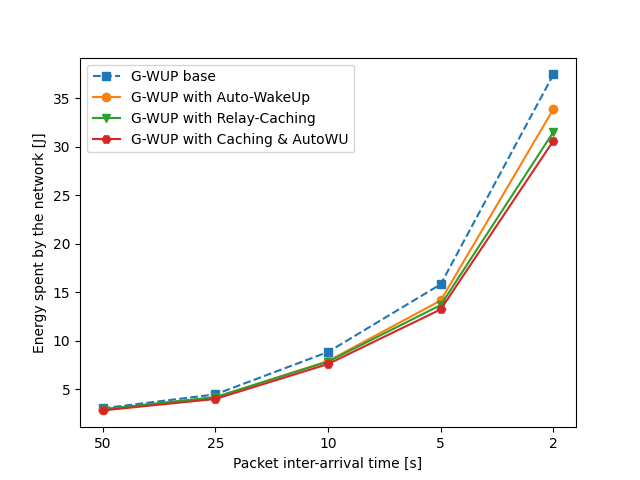
\includegraphics[width=1.1\linewidth]{Contents/Images/graphs/final/energySpent.png}
    \caption{Energy Consuption}
    \label{fig:EnergySpent_final}
  \end{subfigure}
  \begin{subfigure}[t]{0.49\linewidth}
    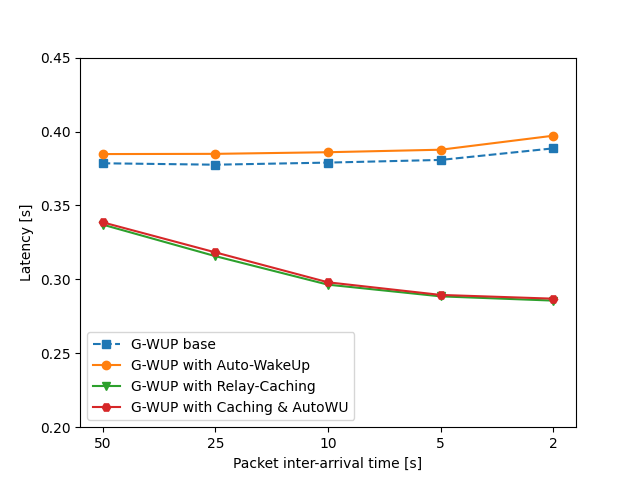
\includegraphics[width=1.1\linewidth]{Contents/Images/graphs/final/latency.png}
    \caption{End-to-End Latency}
    \label{fig:Latency_final}
  \end{subfigure}
  \begin{subfigure}[t]{0.49\linewidth}
    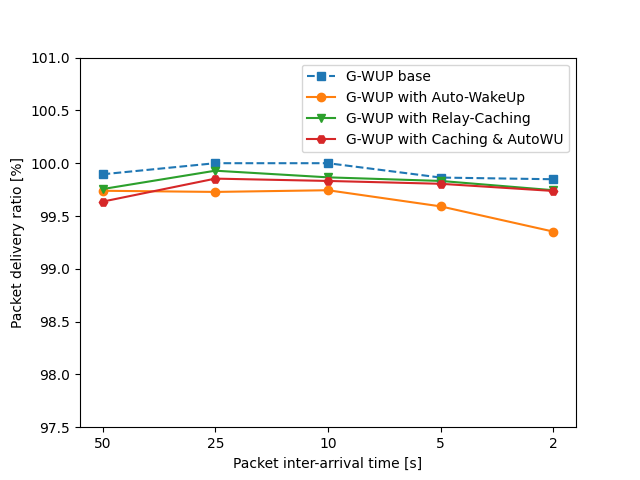
\includegraphics[width=1.1\linewidth]{Contents/Images/graphs/final/pdr.png}
    \caption{Packet Delivery Ratio}
    \label{fig:PDR_final}
  \end{subfigure}
  \caption{Confronto delle prestazioni tra versione base di GreenWUP (blu) e le varianti proposte}
  \label{fig:final}
\end{figure}

La versione All-in-One è quindi efficace nel ridurre la latenza e il consumo energetico di GreenWUP, ad un prezzo di un leggero degrado delle prestazioni in termini di packet delivery ratio.

\subsection{All-in-One 2.0}
Si precisa che tutti in tutti gli scenari simulati si assume che la rete sia completamente connessa per cui da un qualsiasi nodo \textit{x} è possibile raggiungere tramite uno o più nodi il nodo \textit{sink}.
\\\\
\textit{1) TX Time}: come mostrato in \textbf{Figura \ref{fig:TXTime_final2.0}}, si è riusciti a migliorare ulteriormente l'invio di pacchetti di wake-up rispetto la normale \textit{All-in-One}. Ovviamente questo miglioramento si ha in quanto essendo dinamico il tempo per cui si usa il caching di un relay e dato che il tetto massimo è maggiore del numero usato nella prima versione di \textit{All-in-One} ci saranno sicuramente meno fasi di Relay-Selection.\\
In particolare si osserva un miglioramento di circa il 47\% rispetto la prima versione di \textit{All-in-One}.
\\\\
\textit{2) Energy Consuption}: come mostrato in \textbf{Figura \ref{fig:EnergySpent_final2.0}}, la gestione dinamica del numero di ritrasmissioni e il Jitter basato sull'energia residua comportano un miglioramento anche nell'energia complessiva consumata dalla rete. Anche qui si ha un miglioramento del 5\% circa, dovuto al fatto che i vari nodi potrebbero evitare molte più volte la fase di Relay-Selection, avviandola solo nei casi in cui il nodo cached potrebbe scaricarsi.
\\\\
\textit{3) End-to-End Latency}: come mostrato in \textbf{Figura \ref{fig:Latency_final2.0}}, anche il ritardo End-to-End migliora rispetto la versione base. Ovviamente gestendo meglio l'energia consumata e non vincolando l'uso del nodo cached a 3 ma riducendolo o aumentandolo a seconda dei casi ci saranno meno ritrasmissioni dovuti a nodi non più disponibili oltre che meno scambi di pacchetti dovuti alla fase di Relay-Selection. \\
In particolare, anche qui, i miglioramenti sono circa del 5-6\% in tutte le varie configurazioni.
\\\\
\textit{4) Packet Delivery Ratio}: come mostrato in \textbf{Figura \ref{fig:PDR_final2.0}}, la percentuale dei pacchetti ricevuti, che era un punto debole della prima versione di \textit{All-in-One}, è migliorata molto. Si ottiene infatti sempre tra il 99.9\% e il 100\% dei pacchetti consegnati, perdendone circa in quantità minime come 2 o 3 solitamente. \\
Gestendo meglio l'energia ci saranno sempre meno nodi indisponibili per cui le probabilità di perdita dei pacchetti diminuiscono.

\begin{figure}[H]
  \begin{subfigure}[t]{0.49\linewidth}
    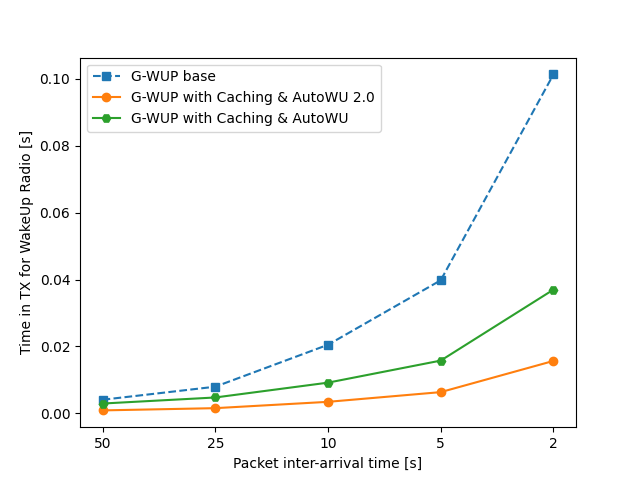
\includegraphics[width=1.1\linewidth]{Contents/Images/graphs/final2.0/tx_time.png}
    \caption{TX Time for the WUR}
    \label{fig:TXTime_final2.0}
  \end{subfigure}
  \begin{subfigure}[t]{0.49\linewidth}
    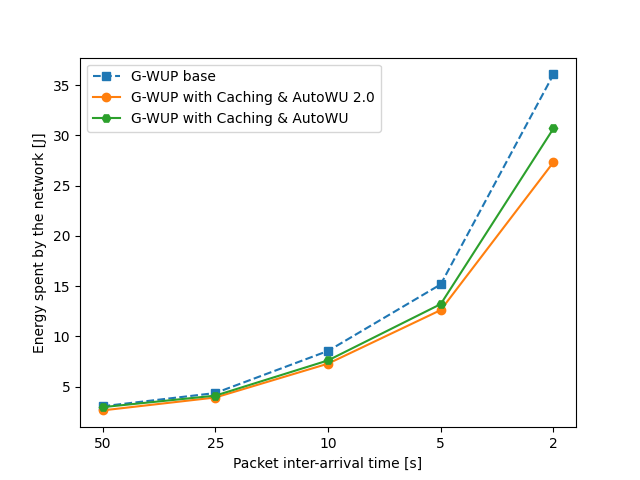
\includegraphics[width=1.1\linewidth]{Contents/Images/graphs/final2.0/energySpent.png}
    \caption{Energy Consuption}
    \label{fig:EnergySpent_final2.0}
  \end{subfigure}
  \begin{subfigure}[t]{0.49\linewidth}
    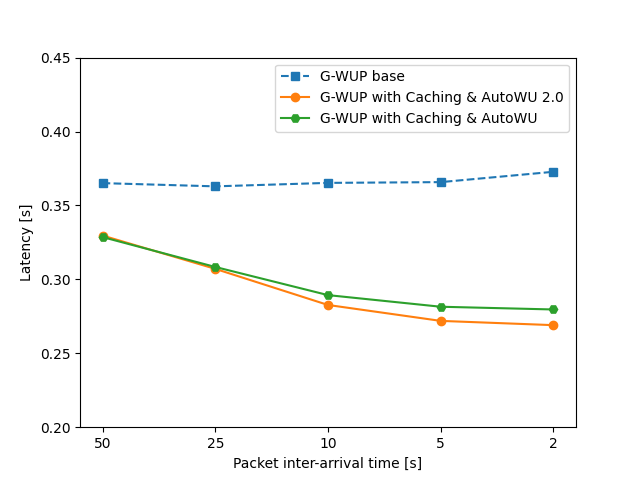
\includegraphics[width=1.1\linewidth]{Contents/Images/graphs/final2.0/latency.png}
    \caption{End-to-End Latency}
    \label{fig:Latency_final2.0}
  \end{subfigure}
  \begin{subfigure}[t]{0.49\linewidth}
    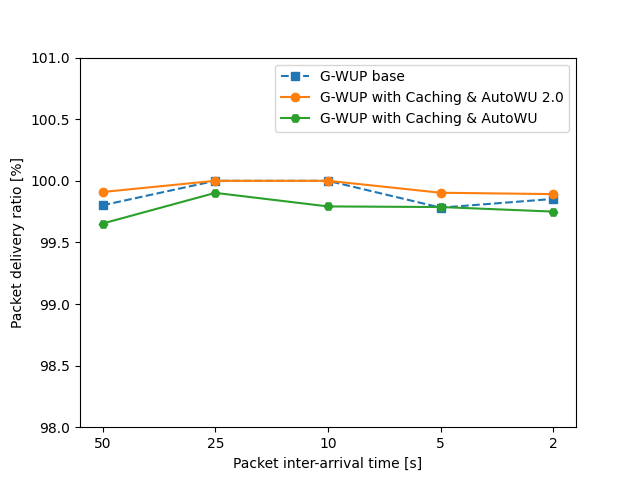
\includegraphics[width=1.1\linewidth]{Contents/Images/graphs/final2.0/pdr.png}
    \caption{Packet Delivery Ratio}
    \label{fig:PDR_final2.0}
  \end{subfigure}
  \caption{Confronto delle prestazioni tra versione base di GreenWUP (blu) e le varianti proposte}
  \label{fig:final2.0}
\end{figure}

La combinazione di tutti i meccanismi proposti consente netti miglioramenti in termini di tutte le metriche prestazionali rispetto al protocollo base. E' efficace nel ridurre al minimo gli onerosi scambi di pacchetti di controllo, consente la scelta dei migliori relay. Questo migliora le prestazioni in termini anche di packet delivery ratio e latenza.
\newpage
\section{Studio prestazionale approfondito dei parametri della variante All-in-One 2.0}
In questo capitolo si andrà a confrontare la proposta finale, ovvero la versione All-in-One 2.0, con la versione base del protocollo GreenWUP con l'obiettivo di studiarne le prestazioni al variare di alcuni parametri come il numero dei nodi, la densità e la fonte di Energy-Harvesting.\\

Sicuramente è interessante vedere come si comportano le due versioni al variare della popolazione della rete e soprattutto non avendo più quell'omogeneità a livello di raccolta di energia, che era invece assunta negli scenari simulativi del precedente capitolo.\\

In particolare, durante i test si continuerà ad usare iaTime di 2, 5, 10, 25, 50 secondi in modo da avere diversi scenari con traffico diverso. Varierà anche, come già detto, il numero di nodi nella rete. Infatti, sono state effettuate simulazioni con 100, 140, 220 nodi in modo da aumentare la densità in rete.\\

Infine, fatto a meno del nodo \textit{sink}, il 50\% dei nodi continuerà ad accumulare energia mediante pannelli solari, mentre l'altra metà dei nodi in rete utilizzerà delle turbine eoliche in modo da avere maggiore eterogeneità tra i componenti della rete.\\

I parametri osservati saranno anche in questo caso la percentuale di pacchetti DATA ricevuti correttamente e il ritardo end-to-end. \\
\newpage

\begin{figure}[h!]
  \begin{subfigure}[t]{0.329\linewidth}
    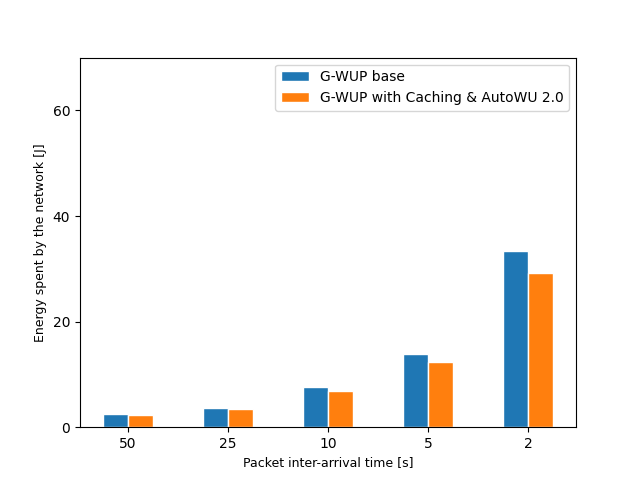
\includegraphics[width=1.13\linewidth]{Contents/Images/graphs/analisi_final2.0/energySpent/energySpent_100.png}
    \caption{100 Nodi}
  \end{subfigure}
  \begin{subfigure}[t]{0.329\linewidth}
    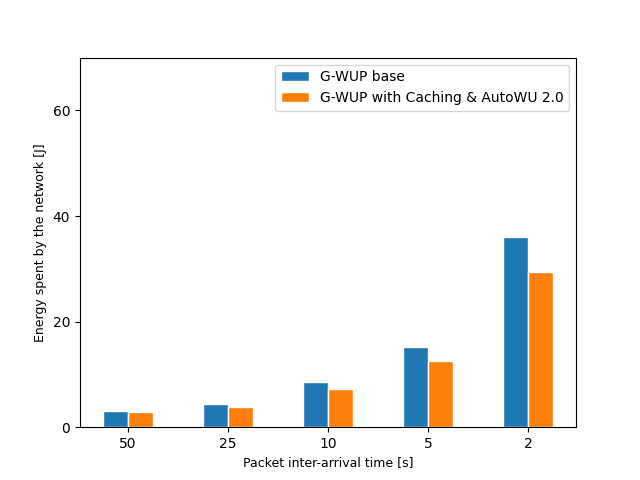
\includegraphics[width=1.13\linewidth]{Contents/Images/graphs/analisi_final2.0/energySpent/energySpent_140.png}
    \caption{140 Nodi}
  \end{subfigure}
  \begin{subfigure}[t]{0.329\linewidth}
    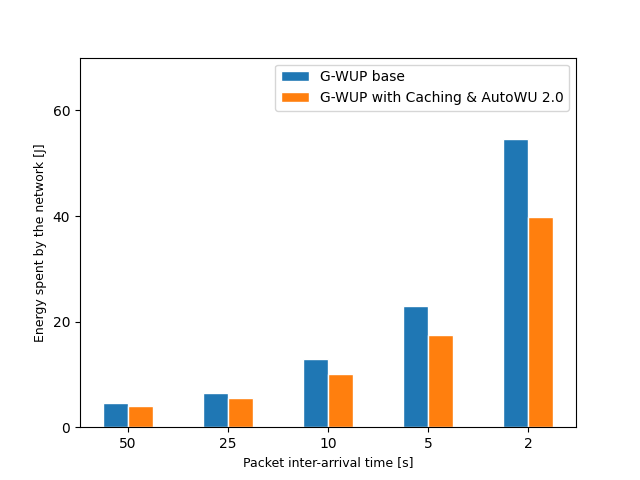
\includegraphics[width=1.13\linewidth]{Contents/Images/graphs/analisi_final2.0/energySpent/energySpent_220.png}
    \caption{220 Nodi}
  \end{subfigure}
  \caption{Risultati ottenuti analizzando l'energia consumata dalla rete}
  \label{fig:analisi_EnergySpent}
\end{figure}

Come mostrato in \textbf{Figura \ref{fig:analisi_EnergySpent}}, la nuova versione di \textit{All-in-One} continua ad ottenere risultati migliori rispetto la versione base di GreenWUP anche cambiando densità e traffico in rete. In particolare dai grafici si evince una crescita dei consumi più lenta rispetto GreenWUP base.\\
Le due proposte, comunque, hanno un comportamento molto simile solo in scenari con poco traffico. Infatti, la differenza di energia aumenta all'aumentare del numero di pacchetti DATA inviati. 

\begin{figure}[h!]
  \begin{subfigure}[t]{0.329\linewidth}
    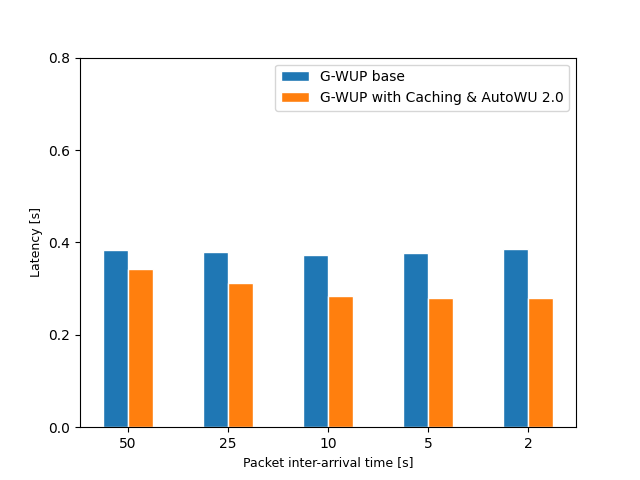
\includegraphics[width=1.13\linewidth]{Contents/Images/graphs/analisi_final2.0/latency/latency_100.png}
    \caption{100 Nodi}
  \end{subfigure}
  \begin{subfigure}[t]{0.329\linewidth}
    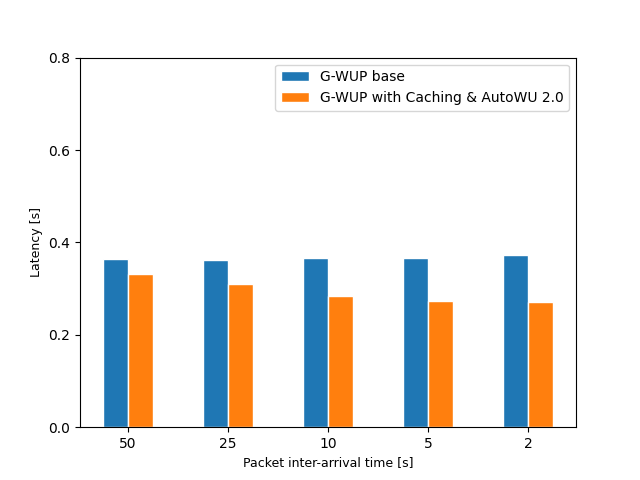
\includegraphics[width=1.13\linewidth]{Contents/Images/graphs/analisi_final2.0/latency/latency_140.png}
    \caption{140 Nodi}
  \end{subfigure}
  \begin{subfigure}[t]{0.329\linewidth}
    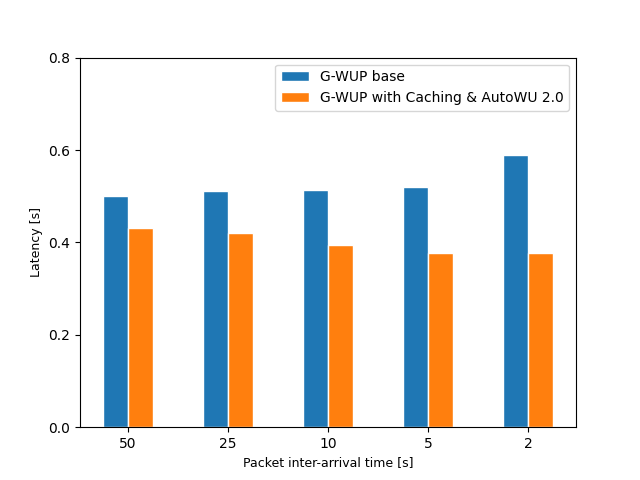
\includegraphics[width=1.13\linewidth]{Contents/Images/graphs/analisi_final2.0/latency/latency_220.png}
    \caption{220 Nodi}
  \end{subfigure}
  \caption{Risultati ottenuti analizzando il ritardo end-to-end}
  \label{fig:analisi_Latency}
\end{figure}

Come mostrato in \textbf{Figura \ref{fig:analisi_Latency}}, anche per il ritardo end-to-end la soluzione proposta risulta essere migliore rispetto alla versione base. \'E possibile notare come all'aumentare del traffico in rete, aldilà della densità della rete, le due versioni di GreenWUP presentino due comportamenti completamente opposti. Infatti per GreenWUP classico il ritardo medio cresce all'aumentare del traffico, mentre per la nuova variante proposta, il ritardo risulta essere minore in scenari in cui il numero di pacchetti DATA è maggiore (proprietà derivante dal caching del next-hop).\\
\newpage

\begin{figure}[h!]
  \begin{subfigure}[t]{0.329\linewidth}
    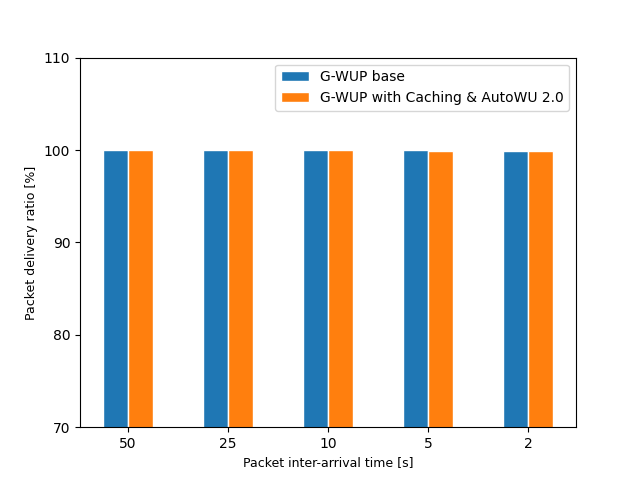
\includegraphics[width=1.13\linewidth]{Contents/Images/graphs/analisi_final2.0/pdr/pdr_100.png}
    \caption{100 Nodi}
  \end{subfigure}
  \begin{subfigure}[t]{0.329\linewidth}
    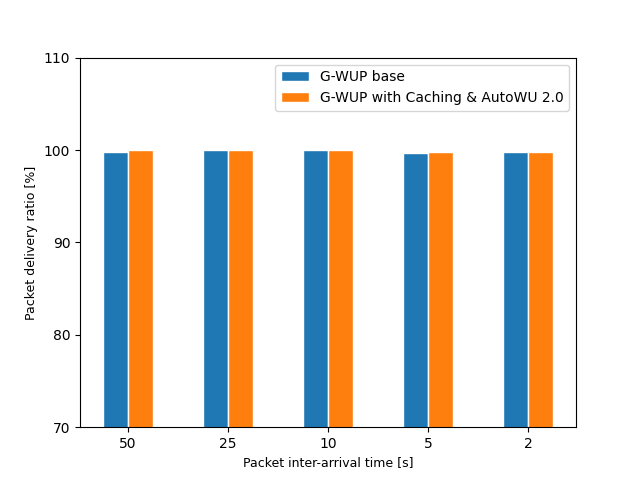
\includegraphics[width=1.13\linewidth]{Contents/Images/graphs/analisi_final2.0/pdr/pdr_140.png}
    \caption{140 Nodi}
  \end{subfigure}
  \begin{subfigure}[t]{0.329\linewidth}
    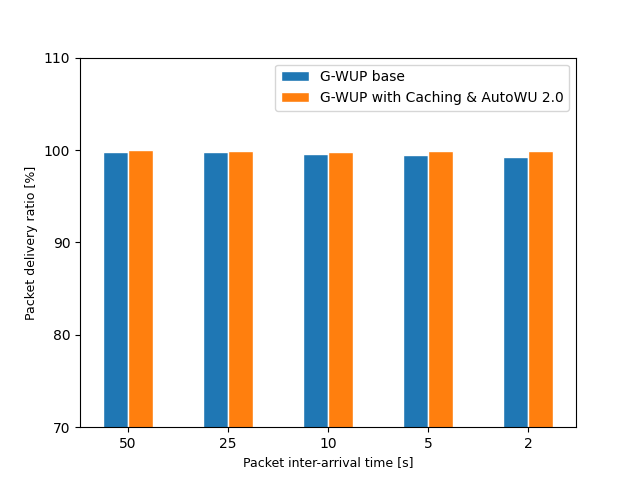
\includegraphics[width=1.13\linewidth]{Contents/Images/graphs/analisi_final2.0/pdr/pdr_220.png}
    \caption{220 Nodi}
  \end{subfigure}
  \caption{Risultati ottenuti analizzando i pacchetti ricevuti correttamente}
  \label{fig:analisi_pdr}
\end{figure}

Come mostrato in \textbf{Figura \ref{fig:analisi_pdr}}, entrambe le soluzioni forniscono sempre una percentuale di pacchetti DATA correttamente ricevuti di almeno il 99\%.\\
Infatti è possibile notare come i risultati siano pressoché identici per le due soluzioni, fatta eccezione per la configurazione con 220 Nodi in cui è possibile vedere un leggero miglioramento rispetto la versione base di GreenWUP nella variante proposta.\\
Sicuramente la migliore gestione dei ritardi e soprattutto dell'energia consumata dalla rete ha fatto il modo di ridurre il numero di pacchetti persi rendendo, di fatto, la variante proposta una valida alternativa alla versione base di GreenWUP.

\chapter{Conclusioni}
Durante questo periodo di tirocinio ho avuto modo di studiare la progettazione di protocolli innovativi per Wireless Sensor Networks, studiando vari aspetti e affrontando le varie problematiche sia a livello teorico che a livello pratico tramite delle simulazioni.\\
Questo ha comportato una fase di studio iniziale delle problematiche delle reti wireless e IoT, non essendo questi temi compresi nei programmi dei corsi della laurea triennale. Ha poi richiesto lo studio della letteratura scientifica del settore per quanto riguarda in particolare protocolli proposti per WSN dotate di wake up radio e energy harvesting.\\

Ho avuto modo di scoprire l'aspetto \textit{green} di queste reti, quindi ho potuto studiare tecnologie come quelle di wake-up e energy-harvesting capendo in che modo queste sono usate nell'ambito dell'IoT.\\

Infine ho avuto modo di approfondire gli aspetti pratici e teorici del protocollo GreenWUP, cercando di trovare alcuni punti deboli e presentare, sia in teoria che in pratica, delle varianti di questo che potrebbero risolvere appunto questi problemi.\\
In particolare ho presentato due varianti paragonando i risultati ottenuti singolarmente da queste con la versione base del protocollo, per poi unire le due proposte in un'unica soluzione e confrontando poi tutti i risultati.\\
Durante questo lavoro di tirocinio, grazie a questo metodo di valutazione sperimentale e confronto prestazionale, è stato possibile vedere come reagiva il protocollo a determinati cambiamenti in modo da concentrare l'attenzione, durante la riprogettazione, su determinati aspetti invece che su altri. \\

In particolare, alla luce dei risultati sopra ottenuti, possiamo notare che la prima soluzione, ovvero Auto-WakeUp, non ha riportato particolari miglioramenti rispetto alla versione base del protocollo. Più interessante invece è stata la seconda proposta, ovvero il Caching dei nodi relay selezionati. Quest'ultima, infatti, ha riportato dei miglioramenti più interessanti in termini di Energia consumata dai nodi della rete e ritardi di latenza.\\

Alla luce di ciò credo che possa essere produttivo andare a modificare la logica di Relay-Selection (come è stato fatto per la variante Relay-Caching), usando magari logiche più complesse come \textit{Reinforcement learning}, piuttosto che andare ad operare su aspetti minori (come è stato invece fatto per la variante Auto-WakeUp). \\
Modifiche come quest'ultima possono avere senso se abbinate a modifiche più importanti, come è stato fatto per la variante finale All-in-one. Questa variante, infatti, risulta essere la migliore in quanto risponde a tutte le inefficienze individuate mediante un'analisi approfondita dei risultati sperimentali e, combinando varie tecniche che affrontino i problemi individuati in modo sinergico, consente di goder di tutti i vantaggi ottenuti con le altre varianti.\\

Mi sono quindi concentrato sull'ottimizzazione della variante All-in-One e, in particolare, di migliorare punti deboli come la staticità del numero di utilizzi di un nodo cached e la logica con cui si calcola il Jitter.\\
\'E stata presentata infatti una nuova variante, \textit{All-in-One 2.0}, con cui sono stati rinforzati questi punti deboli riuscendo ad ottenere miglioramenti in tutte le metriche osservate.\\

In fine si è analizzato nel dettaglio l'ultima versione, ovvero \textit{All-in-One 2.0}, studiando il comportamento cambiando parametri come il numero di nodi nella rete, la densità della rete, studiando come variano le prestazioni e aggiungendo eterogeneità tra i nodi cambiando sorgente di raccolta energia.\\

Il lavoro svolto ha messo in evidenza il potenziale di ottimizzazione del protocollo. Altri studi potrebbero riguardare l'ottimizzazione automatica di alcuni parametri. Sarebbe inoltre interessante estendere il confronto prestazionale ad altri schemi presenti in letteratura.\\

Sarebbe infine interessante, una volta ottimizzate al massimo le varianti proposte, sperimentare le prestazioni mediante un testbed in ambiente reale per reti IoT dotate di WakeUp Radio come quello ideato da SENSES Lab.

\bibliographystyle{siam}
\bibliography{Contents/bibliography}

\end{document}
